\documentclass[11pt]{article}
\usepackage[margin=1in]{geometry}
\usepackage[T1]{fontenc}
\usepackage{lmodern}
\usepackage{amsmath}
\usepackage{mathtools}
\usepackage{amssymb}
\usepackage{amsthm}
\usepackage{microtype}
\usepackage{enumitem}
\usepackage{booktabs}
\usepackage{array}
\newcolumntype{L}[1]{>{\raggedright\arraybackslash}p{#1}}
\usepackage{tikz}
\usetikzlibrary{arrows.meta,positioning,calc}
\usepackage{natbib}
\usepackage[colorlinks=true,linkcolor=blue!50!black,citecolor=green!35!black,urlcolor=blue!60!black]{hyperref}

\newcommand{\R}{\mathbb{R}}
\newcommand{\ip}[2]{\langle #1,#2\rangle}
\newcommand{\norm}[1]{\lVert #1\rVert}
\newcommand{\St}{\operatorname{St}}
\newcommand{\ord}{\operatorname{ord}}
\newcommand{\rank}{\operatorname{rank}}
\newcommand{\TS}{\textsf{TS}}
\newcommand{\SO}{\textsf{SO}}
\newcommand{\ts}[1]{[\TS, #1]}
\newcommand{\so}[1]{[\SO, #1]}
\newcommand{\Clk}{\mathcal{C}}

\theoremstyle{definition}
\newtheorem{theorem}{Theorem}[section]
\newtheorem{proposition}[theorem]{Proposition}
\newtheorem{lemma}[theorem]{Lemma}
\newtheorem{corollary}[theorem]{Corollary}
\newtheorem{definition}[theorem]{Definition}
\newtheorem{remark}[theorem]{Remark}
\newtheorem{example}[theorem]{Example}
\newtheorem{budgetrule}[theorem]{Rule}
\newtheorem{observation}[theorem]{Observation}
\numberwithin{equation}{section}

\title{Saddle-to-saddle dynamics of tree tensor networks\\ on the balanced manifold}
\author{}
\date{Research note, \today}

\begin{document}
\maketitle

\begin{abstract}
We study gradient flow on tree tensor networks (TTNs) trained from a small initialization on a target that is a sum of orthonormal basis tensors. We combine two notes: the main note (\TS), which solves the balanced dynamics of a three-core TTN and reduces rank-one channels on any tree to an orientation flow and quadratures, and the saddle-order note (\SO), which computes the order of the saddle at which one component of the target has been learned. On the three-core model the two describe the same saddles: the Hessian block of \SO{} has the linear rates of \TS, and the order-three descent of \SO{} is the creation of a mode in \TS. We then find an exact invariant manifold of the flow on any tree, carrying a learned channel and one dormant channel on a Steiner subtree. On it the flow reduces to three amplitudes and an orientation flow, and exact identities show that both channels run on a common clock, set by the cores they share. We solve the orientation flow of the dormant channel in closed form for any number of input-carrying cores. For a two-component target this describes the whole saddle-to-saddle trajectory: the escape time from the saddle, with an explicit geometric factor; the plateau between the two acquisitions, which recovers the leading-order law of \SO{} and extends it to non-aligned starts; the duration and end state of the transition, in which the shared cores rebalance; and the resulting change in the clocks of components not yet learned. For targets with more components we state a conjectural budget rule: a dormant channel that sees a single component is acquired when its own clock exhausts a budget. Under the conditions of \SO, at a saddle with one learned component, components are then acquired in order of locality on the tree before order of weight. A learned component can also serve as a stepping stone for later ones, so budgets must be recomputed at each saddle, and a dormant channel that sees several components is acquired as the strongest of them. Simulations of full TTNs confirm the exact statements to integration accuracy, the asymptotic ones with bounded remainders, and the budget rule to $0.02\%$ in isolated three-component examples. They also show long stalls when the bond dimension equals the rank of the target. We end with research questions.
\end{abstract}

\tableofcontents

%======================================================================
\section{Introduction and summary}\label{sec:intro}
%======================================================================

From a small initialization, gradient flow on a deep linear network (DLN) learns the singular modes of its target one at a time, and stalls near a saddle point before each \citep{saxe2014exact,jacot2021saddle}. All plateaus have the same exponent, $\sigma^{-(K-2)}$ for a depth $K$ and an initialization scale $\sigma$, because every mode needs every layer. Tree tensor networks also learn from a small initialization in a saddle-to-saddle fashion \citep{razin2022implicit,furman2026benign}, but each of their cores sees only some of the inputs. Once a first component of the target has been learned, most cores are large, and the next component only needs the cores of a subtree to grow from small values. The saddle-order note (\SO) makes this precise. At the saddle at which one basis-tensor component $j$ has been learned, the order of the saddle is the number $k_r$ of cores of the smallest subtree that connects the cores on which an unlearned component $r$ differs from $j$, and the plateau before $r$ lasts a time proportional to $\sigma^{-(k_r-2)}$, or to $\log(1/\sigma)$ if $k_r=2$ \so{Theorem~1 and eq.~(10)}.

The main note (\TS) approaches the same flow from the opposite end. On the balanced manifold, where the conserved quantities of the flow vanish, it solves the dynamics of a three-core TTN for aligned modes and for a non-aligned channel of bond rank one, reduces a rank-one channel of any tree to an autonomous orientation flow and quadratures, and computes the linear rates of the three-core model at its critical points \ts{Sections~3.6 and~4}.

This note combines the two to describe a whole saddle-to-saddle trajectory on the balanced manifold, both near the saddles, where the plateaus are spent, and away from them, during the transitions. Each statement is labelled as exact, as a leading-order asymptotic, as an approximation, or as a numerical observation. The numerical checks, in \texttt{checks/s2s\_checks.py} and \texttt{checks/s2s\_symbolic.py}, are summarized in Section~\ref{sec:numerics}.

\subsection{Main results}\label{sec:results}

Throughout, the target is $W^\star=\sum_rs_rU_r$, a sum of distinct products of standard basis vectors with weights $s_r>0$, as in \SO; $K$ is the number of cores, $\sigma$ the initialization scale, $j$ the component learned first, and, for a component $r$, $S$ is the Steiner subtree of the cores on which $r$ differs from $j$, with $k=|S|$ cores (Section~\ref{sec:setting}).

\begin{enumerate}[label=\textbf{R\arabic*.},leftmargin=*,itemsep=3pt]
\item \textbf{The two notes describe the same saddles} (Section~\ref{sec:dictionary}). The three-core model of \TS{} is the binary tree with four sites of \SO. At its saddle with one learned mode, the rotation block $H_{\rm rot}=s_j^{1/3}(s_jI-M_1)$ of \SO{} has exactly the rates of \ts{Proposition~4.4(iii)--(iv)}; the descent of order two is the hyperbolic instability of \TS{} (an unlearned mode stronger than the learned one), and the descent of order three along a new channel is the degenerate creation of a mode, with the same escape time. \TS{} contributes what \SO{} does not compute: balance, the motion of the dormant directions, and a geometric factor in the escape time. \SO{} contributes what a three-core model cannot show: the order depends on the tree.

\item \textbf{An exact reduction on any tree} (Proposition~\ref{prop:two-channel}). For a target $s_jU_j+s_rU_r$, possibly with further components that differ from $U_j$ on at least two cores outside $S$, the set of parameters with one learned channel on all cores and one dormant channel on $S$ is invariant under gradient flow. On it the flow reduces to three amplitudes, $a$ for the learned channel off $S$, $x$ for the learned channel on $S$ and $b$ for the dormant channel, and to the directions of the dormant channel on the cores of $S$ that carry inputs. On the balanced manifold, $a^2=x^2+b^2$: the cores off $S$ are shared by both channels.

\item \textbf{A common clock} (Proposition~\ref{prop:clock}). With $\Clk(t):=\int_0^ta^{K-k}$, exactly,
\[
\frac{d}{d\Clk}x^{-(k-2)}=-(k-2)(s_j-\omega_j),\qquad\frac{d}{d\Clk}b^{-(k-2)}=-(k-2)(\rho-\omega_r),
\]
where $\omega_j$ and $\omega_r$ are the amplitudes of the two channels and $\rho$ is the signal seen by the dormant one. Both channels run on the clock $\Clk$, which is set by the $K-k$ shared cores, and the direction of the dormant channel follows an autonomous flow in a time that is a function of $\Clk$ alone. While $j$ is being learned, the dormant channel therefore grows and rotates on the same clock. This is the origin of the factor $1-s_r/s_j$ in the plateau law of \SO, and the identities make that law exact up to $O(1)$ in the clock $\Clk$.

\item \textbf{Closed-form alignment and the geometric factor} (Proposition~\ref{prop:orientation}). For the signal of a basis component, we solve the orientation flow for any number $m$ of input-carrying cores in $S$ (\TS{} solved it for $m=2$ and treated equal overlaps for $m\ge3$): each overlap $p_v$ of the dormant direction with its target satisfies $1-p_v(\tau)^2=(1-p_v(0)^2)\,e^{-2\int_0^\tau\rho}$. The escape time involves
\[
I_\kappa=\frac1{s_r}\int_0^1u^{\kappa-1}\prod_v\big(1-c_vu^2\big)^{-1/2}du,\qquad c_v=1-p_v(0)^2,\quad\kappa=k-2,
\]
which equals $1/(\kappa s_r)$ for an aligned start. Misalignment multiplies it by a factor of order $D^{(m-2)/2}$ when the overlaps are of order $D^{-1/2}$, $D$ being the dimension of the physical legs, and $m\ge3$; for $k=2$ it adds the shift $\Lambda=\log(2/(p_1+p_2))$ to $\log(1/b(0))$.

\item \textbf{Escape times and plateaus} (Corollaries~\ref{cor:escape} and~\ref{cor:plateau}, leading order). From the saddle with a dormant amplitude $\delta$, the escape takes $\delta^{-(k-2)}I_{k-2}/s_j^{(K-k)/K}$ for $k\ge3$, and $[\log(1/\delta)+\Lambda]/(s_rs_j^{(K-2)/K})$ for $k=2$. From a balanced initialization of scale $\sigma$, the plateau between the acquisitions of $j$ and of $r$ lasts
\[
\Delta t\simeq\sigma^{-(k-2)}\,\frac{I_{k-2}-1/((k-2)s_j)}{s_j^{(K-k)/K}},
\]
which is the law (10) of \SO{} for an aligned start, $I_{k-2}=1/((k-2)s_r)$, and extends it to non-aligned starts.

\item \textbf{Transitions} (Section~\ref{sec:away}). A transition between two saddles takes a time that does not depend on $\sigma$, and it ends at the rebalanced state $a_*=(s_j^{2/k}+s_r^{2/k})^{k/(2K)}$ (exact): the shared cores grow and the cores of the learned channel on $S$ shrink. Learning even a weak component moves the shared cores by a relative amount of order $(s_r/s_j)^{2/k}$, which is not small for moderate $k$. If the learned channel follows adiabatically, the transition reduces to a scalar equation, accurate to $0.3\%$ in our tests. If moreover $(s_r/s_j)^{2/k}\ll1$, it is the learning curve of an isolated network of depth $k$, $\dot\omega_r=k\,c^{2/k}\omega_r^{2-2/k}(s_r-\omega_r)$ with $c=s_j^{(K-k)/K}$. The first acquisition after $j$ changes the clocks of the components not yet learned by an explicit factor (Proposition~\ref{prop:clock-change}): it speeds up those whose subtree contains $S$ and slows down those in disjoint parts of the tree.

\item \textbf{Saddle-to-saddle sequences: a conjectural budget rule} (Section~\ref{sec:sequences}). For a two-component target, R2--R6 describe the whole trajectory. For more components we state a conjecture. A dormant channel that sees a single component $r$ (a residual-isolated channel, the analogue of the condition in R2) has a clock $\Clk_r(t)$, the time integral of the product of the learned entries that it uses outside its subtree, and a budget $B_r$, fixed by its amplitude and direction. It is acquired when $\Clk_r$ reaches $B_r$. In our simulations of three-component targets with isolated channels, this holds to within $0.02\%$ for $k_r\ge4$, including after a change of clock rate. The rule needs two qualifications. A dormant channel that sees several components, as in the three-core model, follows the orientation flow of the whole residual it sees, is acquired as the strongest of them, and has a budget computed from that flow. And when a learned component opens a shorter path, a \emph{stepping stone} (Proposition~\ref{prop:relative-order}), budgets must be recomputed at that saddle; in our example the flow finds the shorter path by itself, and the plateau becomes $275$ times shorter. Under the conditions of \SO, at a saddle with one learned component and for dormant amplitudes proportional to $\sigma$, the next component as $\sigma\to0$ is the one with the smallest $k_r$, whatever its weight: locality comes before weight, and weights decide only between components of equal order or above a crossover scale. The same target is therefore learned in different orders by different trees. Finally, in a pilot experiment, a bond dimension equal to the rank that the target needs on a bond stalled the last component for very long times, and one spare bond direction removed the effect.
\end{enumerate}

\subsection{Assumptions and what they mean}\label{sec:assumptions}

\begin{enumerate}[label=\textbf{A\arabic*.},leftmargin=*,itemsep=3pt]
\item \textbf{Population loss with whitened, independent inputs}, $\mathcal L=\tfrac12\norm{W-W^\star}^2$ \ts{Section~3.2}. The data geometry is trivial, and all the structure comes from the target and the tree. Correlated inputs replace $W^\star$ by a moment tensor during the escapes and change the optimum \ts{Section~4.6}; they are not treated here.
\item \textbf{Basis-tensor targets}, as in \SO. The components are products of standard basis vectors with distinct index strings. They are therefore orthonormal and interact only through the network, and their locality on a tree is measured by Steiner subtrees. This idealizes a teacher whose atoms are aligned with a known basis; general teachers, with rotated or entangled atoms, are not covered.
\item \textbf{Balance.} The conserved quantities of the flow vanish. In general, balance equates Gram matrices across each bond, not the amplitudes of individual channels; on the two-channel manifold of R2 it means that each channel has equal amplitudes on the cores where it is alone, and that the shared cores carry the sum of the squares of both channels. A small random initialization is balanced only up to $O(\sigma^2)$, which is the order of the squared dormant amplitudes themselves; Remark~\ref{rem:unbalanced} gives the budget of an unbalanced, aligned dormant channel. Exact balance also freezes channels that are absent at initialization \ts{Remark~3.11(ii)}, so we assume that every dormant channel needed is present at initialization.
\item \textbf{One dormant channel per candidate component}, with a rank-one structure on its Steiner subtree, as on the invariant manifold of R2. With large bond dimensions, several dormant channels per bond coexist after a random initialization; we assume that one of them dominates.
\item \textbf{Two-component targets for the exact statements.} The statements about more components are conjectural and use three further assumptions. (i) \emph{Residual isolation}: each dormant channel sees a single component, i.e.\ every other unlearned component differs from the learned one on at least two cores outside its subtree, as in R2. (ii) \emph{The conditions of \SO{} at a one-component saddle}: $\mu_\ell<s_j$ for every $\ell<k^*/2$, so that neither rotations nor mixed descents beat the new channels, together with the nondegeneracy and edge-capacity conditions of \so{Theorem~1}. For two components (ii) holds when the larger one is learned first \so{Corollary~1(iii)}. (iii) Dormant channels do not interact while they are small.
\item \textbf{Small initialization}, $\sigma\to0$, for the asymptotic statements: the dormant amplitudes are $b_r(0)=c_r\sigma$ with fixed constants $c_r>0$, and the dormant directions lie in the basin of their target, i.e.\ the products of overlaps are positive (Proposition~\ref{prop:orientation}(v) treats the other case). The plateaus, of order $\sigma^{-(k-2)}$ or $\log(1/\sigma)$, are then long compared with the transitions, which are of order one.
\item \textbf{Enough bond dimension}: $\chi_e\ge2$ on the edges of a Steiner subtree for one dormant channel, and enough unused indices for all dormant channels at once. Section~\ref{sec:capacity} suggests that a spare direction beyond the rank required by the target also matters.
\end{enumerate}

\paragraph{Outline.} Section~\ref{sec:setting} sets up the notation of both notes. Section~\ref{sec:dictionary} relates them. Section~\ref{sec:two-channel} introduces the invariant two-channel manifold, Section~\ref{sec:near} analyses the plateaus, Section~\ref{sec:away} the transitions, and Section~\ref{sec:sequences} whole saddle-to-saddle sequences. Section~\ref{sec:numerics} collects the numerical evidence and Section~\ref{sec:questions} the research questions. Proofs are in Appendix~\ref{app:proofs}.

%======================================================================
\section{Setting}\label{sec:setting}
%======================================================================

\subsection{Tree tensor networks and gradient flow}

Let $T$ be a tree with $K$ nodes. Node $v$ holds a core $G_v$, a tensor with one leg for each edge at $v$ and possibly a physical leg of dimension $D_v$; the leg of an edge $e$ has the bond dimension $\chi_e$. Contracting all edge legs gives $W(\theta)\in\bigotimes_v\R^{D_v}$, where $\theta$ collects all core entries and the product runs over the cores with a physical leg. In \SO{} the inputs are $N$ sites of dimension $d$ and core $v$ carries $n_v$ of them, $D_v=d^{n_v}$; the matrix product state (MPS) has one site per core, the hierarchical Tucker (HT) tree one site per leaf and none on internal cores. The loss is
\begin{equation}\label{eq:loss}
\mathcal L(\theta)=\tfrac12\norm{W(\theta)-W^\star}^2,
\end{equation}
the population square loss for whitened independent inputs, and we study the gradient flow $\dot\theta=-\nabla\mathcal L(\theta)$.

\paragraph{Conserved quantities and balance.} For an edge $e=\{u,v\}$, let $G_u^{\langle e\rangle}$ be the matricization of $G_u$ with the leg of $e$ as columns. Then
\begin{equation}\label{eq:Q}
Q_e:=G_u^{\langle e\rangle\top}G_u^{\langle e\rangle}-G_v^{\langle e\rangle\top}G_v^{\langle e\rangle}\in\R^{\chi_e\times\chi_e}
\end{equation}
is constant along gradient flow. This is the TTN version of the balance of deep linear networks \citep{du2018algorithmic}, proved for the three-core model in \ts{Proposition~3.6}; it follows from the invariance of $W$ under $G_u\mapsto G_u^{\langle e\rangle}g$, $G_v\mapsto g^{-1}G_v^{\langle e\rangle}$. The \emph{balanced manifold} is the invariant set on which $Q_e=0$ for every edge.

\subsection{Basis targets, saddles and their order}\label{sec:so-recap}

Following \so{Section~2}, the target is
\begin{equation}\label{eq:target}
W^\star=\sum_rs_rU_r,\qquad U_r=\bigotimes_ve_{\pi_r(v)},\qquad s_r>0,
\end{equation}
where $\pi_r$ is a string of basis indices, one per site, and $e_{\pi_r(v)}\in\R^{D_v}$ is the basis vector that $U_r$ has on the sites of core $v$. Distinct strings make the $U_r$ orthonormal. Fix a learned component $j$, write $q_v:=e_{\pi_j(v)}$, and let $\theta_j$ ($\theta_S$ in \SO) be the point with cores $G_v=a_vq_v\otimes e_0\otimes\dots\otimes e_0$, $\prod_va_v=s_j$, so that $W(\theta_j)=s_jU_j$ through one channel, index $0$, on every edge. The points of this form are related by diagonal gauge transformations, and we use the balanced one, $a_v=s_j^{1/K}$. For $r\neq j$, let
\begin{equation}\label{eq:Vr}
V_r:=\{v:\ \text{the strings }\pi_r\text{ and }\pi_j\text{ differ on the sites of }v\},\qquad S_r:=\St(V_r),\qquad k_r:=|S_r|,
\end{equation}
where $\St(B)$ is the smallest subtree containing $B$ (the Steiner subtree), and $k^*:=\min_{r\neq j}k_r$. The point $\theta_j$ is critical if and only if $k^*\ge2$ \so{Lemma~1}. Its \emph{order} is the exponent of the fastest local decrease of the loss, $\min_{\norm{\theta-\theta_j}\le\epsilon}\mathcal L(\theta)-\mathcal L(\theta_j)\sim-c\,\epsilon^{\ord}$.

\SO{} computes this order. A new channel along $S_r$, with entries of size $\epsilon$ on its $k_r$ cores, lowers the loss by $s_rs_j^{(K-k_r)/K}\epsilon^{k_r}$ \so{eq.~(5)}. Combined perturbations, built from rotations of single cores and from new channels on smaller subtrees, are recorded in coupling matrices $M_\ell$, with largest eigenvalues $\mu_\ell$ and $\ell^*:=\min\{\ell:\mu_\ell>s_j\}$ \so{Definition~1}. For $\ell=1$, the Hessian block of the rotations is
\begin{equation}\label{eq:Hrot}
H_{\rm rot}=s_j^{(K-2)/K}\big(s_jI-M_1\big)\qquad\text{at the balanced point \so{eq.~(8)}}.
\end{equation}
\begin{theorem}[\SO, Theorem~1]\label{thm:so}
Under mild nondegeneracy and bond-dimension conditions, $\ord(\theta_j)=\min(k^*,2\ell^*)$. In particular, for $W^\star=s_jU_j+s_rU_r$ with $s_r<s_j$, the order is $k_r$.
\end{theorem}
\SO{} then derives, at leading order and without proof, the escape time from $\theta_j$ along a descent of order $p$ with coefficient $c$ from a perturbation of size $\delta$, $\log(1/\delta)/c$ for $p=2$ and $\delta^{-(p-2)}/((p-2)c)$ for $p\ge3$ \so{eq.~(9)}, and, for two components from an aligned initialization of scale $\sigma$, the plateau between the acquisitions of $j$ and $r$:
\begin{equation}\label{eq:so10}
\Delta t\simeq\frac{1-s_r/s_j}{s_rs_j^{(K-2)/K}}\log\frac1\sigma\quad(k_r=2),\qquad\Delta t\simeq\frac{1-s_r/s_j}{(k_r-2)s_rs_j^{(K-k_r)/K}}\,\sigma^{-(k_r-2)}\quad(k_r\ge3).
\end{equation}

\subsection{The three-core model}\label{sec:three-core}

The model of \ts{Section~3} is $M=ACB^\top$, with a core $A$ carrying the legs $\{1,2\}$, a core $B$ carrying the legs $\{3,4\}$, and an internal core $C$. This is the binary tree with four sites of \SO: two bottom cores with two sites each and a root without sites. A basis target is a matrix with the entries $s_r$ at the positions $(\pi_r(1,2),\pi_r(3,4))$. A component that shares its row or its column with $j$ differs from $j$ on a single core, $k_r=1$, and $\theta_j$ is then not critical. If all components have distinct rows and columns, $k_r=3=K$ for all $r$, and the singular value decomposition of $M^\star$ is in the standard basis, with singular values $s_r$.

%======================================================================
\section{How the two notes fit together}\label{sec:dictionary}
%======================================================================

Table~\ref{tab:dictionary} lists the correspondences. The next proposition checks the central one.

\begin{table}[htbp]
\centering
\footnotesize
\renewcommand{\arraystretch}{1.25}
\begin{tabular}{L{0.3\textwidth}L{0.3\textwidth}L{0.31\textwidth}}
\toprule
\SO{} (any tree, basis targets) & \TS{} (three-core model, balanced) & Relation \\
\midrule
binary tree with four sites, $K=3$ & $M=ACB^\top$, single cut $\{1,2\}|\{3,4\}$ & identical \\
saddle $\theta_j$, one channel per edge & critical point $M_{\{j\}}$ & identical (balanced gauge) \\
unused channels, $\chi_e-1$ per edge & bond directions outside $\operatorname{range}C$; absent modes & on the balanced manifold, a channel absent at $t=0$ stays absent \ts{Remark~3.11(ii)} \\
$H_{\rm rot}=s_j^{1/3}(s_jI-M_1)$ & rates of \ts{Proposition~4.4(iii),(iv)} & $H_{\rm rot}$ has eigenvalues minus these rates (Proposition~\ref{prop:dictionary}) \\
order $2$ ($\mu_1>s_j$) & hyperbolic saddle (learned mode weaker than an unlearned one) & identical \\
order $k_r=3$, new channel along $\St(V_r)$ & creation of a mode; degenerate & identical \\
escape law (9), $p=3$: $1/(s_r\delta)$ & $t_\eta=I/s(0)+O(1)$ \ts{Corollary~4.3} & \TS{} adds the factor $s_rI\ge1$ \\
plateau law \eqref{eq:so10}, $k_r=K=3$ & independent aligned modes \ts{Proposition~3.10} & no shared core: $\Delta t=(1/s_r-1/s_j)/\sigma$ \\
order $k_r=|\St(V_r)|\le K$ & rank-one channel of any tree, escape $\propto s(0)^{-(N-2)}$ \ts{Section~4.7} & \TS{} treats the escape from the origin; \SO{} the later saddles \\
--- & balance, $Q_e$, rank freezing & \SO{} uses balance only as a gauge choice \\
\bottomrule
\end{tabular}
\caption{Dictionary between the saddle-order note (\SO) and the main note (\TS).}
\label{tab:dictionary}
\end{table}

\begin{proposition}[The two analyses agree on the three-core model]\label{prop:dictionary}
Let $K=3$, let both bond dimensions be at least $2$, and let the components of $W^\star$ have distinct rows and columns (Section~\ref{sec:three-core}), with $s_r\neq s_j$ for every $r\neq j$; let $j$ be learned at the balanced point.
\begin{enumerate}[label=(\roman*),nosep]
\item $M_1$ couples the rotation of $A$ towards the row of $r$ with the rotation of $B$ towards the column of $r$, with weight $s_r$, for every $r\neq j$, and has no other entries. Its eigenvalues are $\pm s_r$, $r\neq j$, and $0$. Hence $H_{\rm rot}$ has the eigenvalues $s_j^{1/3}(s_j-s_r)$, $s_j^{1/3}(s_j+s_r)$ and $s_j^{4/3}$, which are minus the rates of \ts{Proposition~4.4(iii),(iv)}, with $\sigma^\star_i=s_j$ and $\sigma^\star_q=s_r$.
\item $k^*=3$ and $\ell^*\in\{1,\infty\}$, so the order of $\theta_j$ is $2$ if some unlearned singular value exceeds $s_j$, and $3$ otherwise: the hyperbolic and the degenerate saddles of \ts{Section~4.3}.
\item The escape law of \SO{} for $p=3$ is the aligned case of \ts{Corollary~4.3}, applied to the dormant channel, which for $K=3$ shares no core with the learned one: $t_\eta=I/s(0)+O(1)$ with $I=1/s_r$.
\end{enumerate}
\end{proposition}

\begin{proof}
(i) A single-core rotation changes the row (rotation of $A$) or the column (rotation of $B$) of $U_j$. A pair of rotations on disjoint cores produces the component $r$ if and only if they move the row and the column of $U_j$ to those of $U_r$, which defines the entries of $M_1$ \so{eq.~(6)}. Each rotation is coupled to at most one other, so $M_1$ is a direct sum of $2\times2$ blocks $\begin{psmallmatrix}0&s_r\\s_r&0\end{psmallmatrix}$ and zeros. Substituting into~\eqref{eq:Hrot} with $K=3$ gives the eigenvalues; in \TS, the same blocks appear as the equations $\dot\varepsilon_L=s_i(\sigma^\star_j\varepsilon_R-\sigma^\star_i\varepsilon_L)$, $\dot\varepsilon_R=s_i(\sigma^\star_j\varepsilon_L-\sigma^\star_i\varepsilon_R)$ in the proof of \ts{Proposition~4.4}. (ii) follows from (i) and Theorem~\ref{thm:so}, whose nondegeneracy condition $\mu_1\neq s_j$ is the assumption $s_r\neq s_j$, and whose capacity condition is the assumption on the bond dimensions; $k^*=3$ restricts $\ell$ to $\ell<3/2$. (iii) For $K=3$ the dormant channel shares no core with the learned one, and for aligned modes the two are exactly decoupled \ts{Proposition~3.10}; \ts{Corollary~4.3} therefore applies to the dormant mode as to a rank-one channel started at amplitude $\delta$, with $I=1/s_r$ for the aligned direction. The descent of order three has the coefficient $s_rs_j^{0}=s_r$, and \so{eq.~(9)} gives the same time, $\delta^{-1}/s_r$.
\end{proof}

\paragraph{What each note contributes.} \SO{} determines the \emph{order} of every saddle visited after one component is learned, on any tree. Its plateau law~\eqref{eq:so10} is derived at leading order, for aligned initializations, and it rests on the assumption that the cores of the learned channel share a common size. \TS{} works on the balanced manifold, where these sizes are fixed by the conserved quantities, and it follows the \emph{directions} of the modes as well as their amplitudes: the escape time of a non-aligned channel carries a geometric factor $I$, which can be large \ts{Corollary~4.3}. But \TS{} solves only the escape from the origin and the three-core model, in which every component needs every core ($k_r=K$) and the plateaus cannot depend on the tree. What is missing on both sides is an exact description of the later saddles on a general tree: the shared cores, the non-aligned dormant directions, the transitions and the sequence. This is the subject of the rest of the note.

%======================================================================
\section{An exact reduction: the two-channel manifold}\label{sec:two-channel}
%======================================================================

Fix the learned component $j$ and a component $r$ with $|V_r|\ge2$; write $S:=S_r$, $k:=k_r\ge2$, $E_S$ for the edges of $S$, and $S_\phi$ for the $m$ cores of $S$ that carry a physical leg. Every leaf of $S$ lies in $V_r$, and so does at least one core of every connected component of $S\setminus\{v\}$, for any $v\in S$. For a core $v$, write $\mathbf e^{(v)}_F$ for the bond multi-index of $v$ that is $1$ on the edges in $F$ and $0$ on the other edges at $v$.

\begin{definition}[Two-channel manifold]\label{def:two-channel}
Assume $\chi_e\ge2$ for $e\in E_S$. The set $\mathcal M_{j,r}$ consists of the parameters
\begin{equation}\label{eq:ansatz}
G_v=a_v\,q_v\otimes\mathbf e^{(v)}_\emptyset\quad(v\notin S),\qquad G_v=x_v\,q_v\otimes\mathbf e^{(v)}_\emptyset+V_v\otimes\mathbf e^{(v)}_{E_S}\quad(v\in S),
\end{equation}
with $a_v,x_v>0$ and vectors $V_v\in\R^{D_v}$ such that $V_v\perp q_v$ for $v\in V_r$; for a core without physical leg, $q_v=1$ and $V_v$ is a scalar. Up to the positivity of $a_v$ and $x_v$, this is a linear subspace of the parameters. Where $V_v\neq0$ we write $V_v=b_vw_v$ with $b_v>0$ and a unit vector $w_v$ ($w_v=1$ for a core without physical leg). The first channel uses index $0$ on every edge; the second uses index $1$ on the edges of $S$ and index $0$ on the edges that leave $S$ (Figure~\ref{fig:two-channel}).
\end{definition}

\begin{figure}[tbp]
\centering
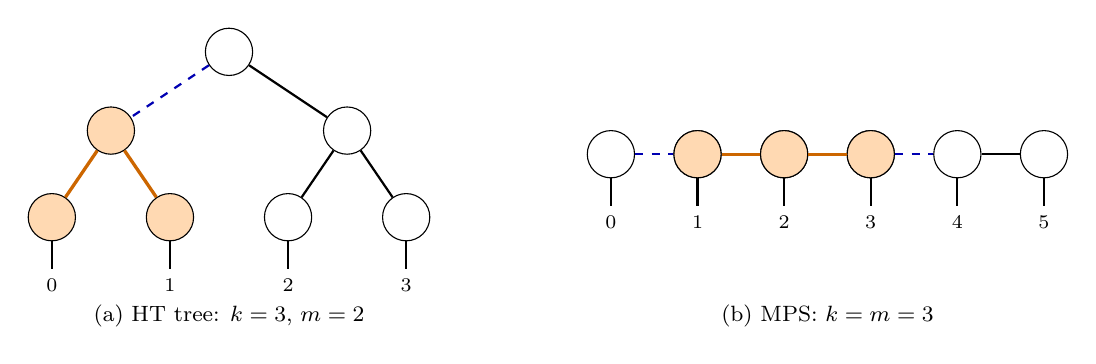
\begin{tikzpicture}[
  core/.style={circle,draw,minimum size=6mm,inner sep=0pt,font=\scriptsize},
  inS/.style={core,fill=orange!30},
  leg/.style={thick},
  sedge/.style={very thick,orange!80!black},
  ledge/.style={thick,blue!70!black,dashed},
  oedge/.style={thick}]
\begin{scope}
\node[core] (r) at (0,0) {};
\node[inS] (a) at (-1.5,-1) {};
\node[core] (b) at (1.5,-1) {};
\node[inS] (l0) at (-2.25,-2.1) {};
\node[inS] (l1) at (-0.75,-2.1) {};
\node[core] (l2) at (0.75,-2.1) {};
\node[core] (l3) at (2.25,-2.1) {};
\draw[ledge] (r)--(a);
\draw[oedge] (r)--(b);
\draw[sedge] (a)--(l0); \draw[sedge] (a)--(l1);
\draw[oedge] (b)--(l2); \draw[oedge] (b)--(l3);
\foreach \n/\s in {l0/0,l1/1,l2/2,l3/3} { \draw[leg] (\n.south)--++(0,-0.35) node[below,font=\scriptsize] {$\s$}; }
\node[font=\footnotesize] at (0,-3.35) {(a) HT tree: $k=3$, $m=2$};
\end{scope}
\begin{scope}[xshift=7.6cm]
\foreach \i in {0,...,5} { \node[core] (m\i) at (\i*1.1-2.75,-1.3) {}; }
\foreach \i in {1,2,3} { \node[inS] at (m\i) {}; }
\draw[oedge] (m4)--(m5); \draw[ledge] (m0)--(m1); \draw[sedge] (m1)--(m2); \draw[sedge] (m2)--(m3); \draw[ledge] (m3)--(m4);
\foreach \i in {0,...,5} { \draw[leg] (m\i.south)--++(0,-0.35) node[below,font=\scriptsize] {$\i$}; }
\node[font=\footnotesize] at (0,-3.35) {(b) MPS: $k=m=3$};
\end{scope}
\end{tikzpicture}
\caption{The two-channel manifold. Shaded cores form the Steiner subtree $S$ of $V_r$: (a) $V_r$ consists of the leaves of sites $0$ and $1$, and $S$ adds their parent, which has no site; (b) $V_r=\{1,3\}$, and $S$ adds core $2$, which carries a site on which $r$ agrees with $j$. The learned channel uses index $0$ on every edge; the dormant channel uses index $1$ on the edges of $S$ (thick) and index $0$ on the edges that leave $S$ (dashed), where it shares the cores of the learned channel. On a dashed edge balance reads $a^2=x^2+b^2$.}
\label{fig:two-channel}
\end{figure}

On $\mathcal M_{j,r}$ the network is
\begin{equation}\label{eq:W-two-channel}
W=\omega_jU_j+\omega_rD,\qquad\omega_j=\prod_{v\notin S}a_v\prod_{v\in S}x_v,\qquad\omega_r=\prod_{v\notin S}a_v\prod_{v\in S}b_v,
\end{equation}
where $D:=\bigotimes_{v\in S_\phi}w_v\otimes\bigotimes_{v\notin S}q_v$ is a unit tensor orthogonal to $U_j$. Indeed, in each term of the contraction the two cores at an edge of $S$ use entries with the same index on that edge, so the cores of $S$, which form a connected set, use either all their first entries or all their second ones; the cores off $S$ have a single entry. The dormant channel sees the signal
\begin{equation}\label{eq:rho}
\rho:=\ip{W^\star}{D}=s_r\,P,\qquad P:=\prod_{v\in S_\phi}p_v,\qquad p_v:=\ip{w_v}{t_v},\quad t_v:=e_{\pi_r(v)}.
\end{equation}
The coefficient of the component $r$ in the network is $\hat\omega_r:=\ip{U_r}{W}=P\,\omega_r$; it is $\hat\omega_r$, not $\omega_r$, that measures the acquisition of $r$.

\begin{proposition}[Invariance and reduced flow; exact]\label{prop:two-channel}
Let $W^\star=s_jU_j+s_rU_r+W'$, where $W'$ is a sum of components $r'$ each of which differs from $U_j$ on at least two cores outside $S$ (possibly $W'=0$). Then $\mathcal M_{j,r}$ is invariant under gradient flow as long as the amplitudes $a_v$ and $x_v$ stay positive, the loss on it is
\begin{equation}\label{eq:reduced-loss}
\mathcal L=\tfrac12(\omega_j-s_j)^2+\tfrac12\omega_r^2-\omega_r\rho+\tfrac12\big(s_r^2+\norm{W'}^2\big),
\end{equation}
and, where all $b_v>0$, the flow reads
\begin{equation}\label{eq:reduced-flow}
\begin{aligned}
\dot a_v&=\frac{\omega_j(s_j-\omega_j)+\omega_r(\rho-\omega_r)}{a_v}\ (v\notin S),&\dot x_v&=\frac{\omega_j(s_j-\omega_j)}{x_v}\ (v\in S),\\
\dot b_v&=\frac{\omega_r(\rho-\omega_r)}{b_v}\ (v\in S),&\dot w_v&=\frac{\omega_r}{b_v^2}\big(I-w_vw_v^\top\big)\nabla_{w_v}\rho\ (v\in S_\phi).
\end{aligned}
\end{equation}
On $\mathcal M_{j,r}$ the conserved quantities~\eqref{eq:Q} reduce to $a_u^2-a_v^2$ on the edges between cores off $S$, to $a_v^2-x_u^2-b_u^2$ on the edges that leave $S$ ($u\in S$), and to $x_u^2-x_v^2$ and $b_u^2-b_v^2$ on the edges of $S$. On the balanced manifold, therefore, $a_v\equiv a$, $x_v\equiv x$, $b_v\equiv b$, with
\begin{equation}\label{eq:balance}
a^2=x^2+b^2,\qquad\omega_j=a^{K-k}x^k,\qquad\omega_r=a^{K-k}b^k.
\end{equation}
When $k=K$ there is no core off $S$; then $\omega_j=x^K$ and $\omega_r=b^K$, and $a:=(x^2+b^2)^{1/2}$ is bookkeeping only, entering through $a^{K-k}=1$.
\end{proposition}

The proof (Appendix~\ref{app:two-channel}) shows that the gradient vanishes at every entry outside the support of~\eqref{eq:ansatz} and preserves $V_v\perp q_v$ on $V_r$. Three facts are used: every connected component of $S\setminus\{v\}$ contains a core of $V_r$, on which $w\perp q$; $|V_r|\ge2$; and the components in $W'$ differ from $U_j$ on two cores outside $S$, so that no single core can produce them.

\begin{remark}[Reading the reduction]\label{rem:reading}
\leavevmode
\begin{enumerate}[label=(\roman*),nosep]
\item \emph{Shared cores couple the channels.} The two channels interact only through the cores off $S$, whose amplitude $a$ is driven by both: by~\eqref{eq:balance}, the bond on an edge that leaves $S$ carries $x^2+b^2$. When $k=K$, as in the three-core model, there is no shared core, the channels decouple, and~\eqref{eq:reduced-flow} gives $\dot x=x^{K-1}(s_j-x^K)$ and $\dot b=b^{K-1}(\rho-b^K)$, i.e.\ \ts{Proposition~3.10} for each mode and \ts{eq.~(4.15)} for the dormant one.
\item \emph{Which cuts change.} Across an edge of $S$, both sides contain cores of $V_r$, and the matricization of $W$ has the two singular values $\omega_j$ and $\omega_r$. Across an edge outside $S$, $U_j$ and $D$ agree on the side away from $S$, and the matricization has rank one, with singular value $(\omega_j^2+\omega_r^2)^{1/2}$. Acquiring $r$ therefore adds a singular value on the edges of $S$, simultaneously on all of them, and increases the leading singular value on all other edges. The edges of $S$ are those on which the rank of the model must grow \so{Section~6, item (2)}.
\item \emph{What the reduction excludes.} The manifold contains one dormant channel. It does not describe several dormant channels sharing entries, rotations of the learned channel towards other components (excluded here by the condition on $W'$), or targets that are not sums of basis tensors.
\end{enumerate}
\end{remark}

%======================================================================
\section{Near the saddle: a common clock and the plateaus}\label{sec:near}
%======================================================================

\subsection{The common clock}

The identities below need balance only inside $S$ ($x_v\equiv x$, $b_v\equiv b$ on $S$); the amplitudes off $S$ may be unbalanced. Define the clock and the orientation time
\begin{equation}\label{eq:clocks}
\Clk(t):=\int_0^tA(t')\,dt',\qquad\tau(t):=\int_0^tA(t')\,b(t')^{k-2}dt',\qquad A:=\prod_{v\notin S}a_v\quad(=a^{K-k}\text{ if balanced}).
\end{equation}

\begin{proposition}[Common clock; exact]\label{prop:clock}
On $\mathcal M_{j,r}$ with balance inside $S$:
\begin{enumerate}[label=(\roman*),nosep]
\item $\dfrac{dx}{d\Clk}=x^{k-1}(s_j-\omega_j)$, $\dfrac{db}{d\Clk}=b^{k-1}(\rho-\omega_r)$, and $\dfrac{dw_v}{d\tau}=\big(I-w_vw_v^\top\big)\nabla_{w_v}\rho$, an autonomous flow on the product of spheres.
\item For $k\ge3$, $\dfrac{d}{d\Clk}x^{-(k-2)}=-(k-2)(s_j-\omega_j)$ and $\dfrac{d}{d\Clk}b^{-(k-2)}=-(k-2)(\rho-\omega_r)$; for $k=2$, $\dfrac{d}{d\Clk}\log x=s_j-\omega_j$ and $\dfrac{d}{d\Clk}\log b=\rho-\omega_r$, and $\tau=\Clk$.
\item Let $\mathcal A(\tau):=\int_0^\tau(\rho-\omega_r)\,d\tau'$ along the trajectory, and $G(\tau):=\int_0^\tau e^{-(k-2)\mathcal A(\tau')}d\tau'$. Then $b=b(0)e^{\mathcal A}$ and
\begin{equation}\label{eq:G-identity}
G(\tau(t))=b(0)^{k-2}\,\Clk(t)\qquad\text{for all }t.
\end{equation}
\end{enumerate}
\end{proposition}

\begin{proof}
(i) follows from~\eqref{eq:reduced-flow}, since $\omega_j/x=Ax^{k-1}$, $\omega_r/b=Ab^{k-1}$ and $\omega_r/b^2=Ab^{k-2}$. (ii) follows from (i). (iii) By (i), $d\log b/d\tau=\rho-\omega_r$, so $b=b(0)e^{\mathcal A}$; then $dG/dt=e^{-(k-2)\mathcal A}\,Ab^{k-2}=b(0)^{k-2}A=b(0)^{k-2}\,d\Clk/dt$.
\end{proof}

Both channels are thus driven on the clock $\Clk$, the time integral of the product of the shared cores. The direction of the dormant channel runs on $\tau$, and by~\eqref{eq:G-identity} its progress is a function of $\Clk$ alone: everything the dormant channel does during a plateau or during the acquisition of $j$ is indexed by $\Clk$. When $j$ is being learned, the shared cores grow and $\Clk$ accelerates, and the dormant channel profits from it in the same way as the learned channel. This is the growth before the plateau of \so{Section~7.6}, which the identities make exact.

\subsection{The orientation of a dormant channel}

The flow of Proposition~\ref{prop:clock}(i) is projected gradient ascent of the multilinear form $\rho=s_r\prod_vp_v$ on a product of $m$ spheres. For $m=2$ it is Oja's flow on the dilation of a rank-one matrix, solved in \ts{Proposition~4.2}; for $m\ge3$, \TS{} reduces it to a single equation for equal overlaps and estimates the alignment time \ts{Section~4.7}. For a rank-one target it can be solved in general.

\begin{proposition}[Orientation flow of a rank-one dormant channel; exact]\label{prop:orientation}
Let $E(\tau):=\exp\big(-2\int_0^\tau\rho\big)$ and $c_v:=1-p_v(0)^2$, and assume $p_v(0)\neq0$ for all $v\in S_\phi$. Flipping the signs of two directions $w_u$ and $w_v$ changes neither $W$ nor the flow; when $P(0)>0$ we use this gauge to make all $p_v(0)>0$.
\begin{enumerate}[label=(\roman*),nosep]
\item $p_v'=s_r\prod_{u\neq v}p_u\,(1-p_v^2)$, the component of $w_v$ orthogonal to $t_v$ keeps its direction, and
\begin{equation}\label{eq:orientation-invariant}
1-p_v(\tau)^2=c_v\,E(\tau)\qquad\text{for every }v\in S_\phi.
\end{equation}
\item If $P(0)>0$, then in this gauge all $p_v$ stay positive, $E$ decreases from $1$ to $0$, $E'=-2s_rE\prod_v(1-c_vE)^{1/2}$, and $p_v\to1$.
\item If $P(0)>0$, then for $\kappa>0$,
\begin{equation}\label{eq:I-kappa}
I_\kappa:=\int_0^\infty E(\tau)^{\kappa/2}d\tau=\frac1{s_r}\int_0^1u^{\kappa-1}\prod_{v\in S_\phi}\big(1-c_vu^2\big)^{-1/2}du,
\end{equation}
and the delay of $\int_0^\tau\rho$ behind its aligned value $s_r\tau$ has the finite limit
\begin{equation}\label{eq:Lambda}
\Lambda:=\lim_{\tau\to\infty}\Big(s_r\tau-\int_0^\tau\rho\Big)=\int_0^1\Big(\prod_{v\in S_\phi}\big(1-c_vu^2\big)^{-1/2}-1\Big)\frac{du}u.
\end{equation}
For equal overlaps $p_v(0)=p$, $I_\kappa=\frac1{\kappa s_r}\,{}_2F_1\big(\tfrac m2,\tfrac\kappa2;\tfrac\kappa2+1;1-p^2\big)$. In all cases $I_\kappa\ge1/(\kappa s_r)$, with equality if and only if the start is aligned.
\item For $m=2$, $E=1/Z$ with $Z$ given by \ts{eq.~(4.7)} for the rank-one teacher, and $\Lambda=\log\big(2/(|p_1(0)|+|p_2(0)|)\big)$.
\item If $P(0)<0$ and the smallest $|p_v(0)|$ is attained once, at $c_{\max}=\max_vc_v$, then $E$ first increases to $1/c_{\max}$, when that overlap crosses zero, and then decreases to $0$; and
\[
I_\kappa=\frac1{2s_r}\Big(\int_1^{1/c_{\max}}+\int_0^{1/c_{\max}}\Big)E^{\kappa/2-1}\prod_v\big|1-c_vE\big|^{-1/2}dE.
\]
\end{enumerate}
\end{proposition}

The proof is in Appendix~\ref{app:orientation}. The variable $u=E^{1/2}=e^{-\int\rho}$ is $b(0)/b$ in the absence of the self-interaction $\omega_r$, so~\eqref{eq:I-kappa} integrates over the growth of the dormant amplitude: $u\approx1$ while the channel searches for its direction, and $u\to0$ as it escapes.

\begin{remark}[Size of the geometric factor]\label{rem:geometric}
For overlaps $p_v(0)^2=1/D$, typical of random directions in physical legs of dimension $D$, the integrand of~\eqref{eq:I-kappa} is concentrated near $u=1$ when $D$ is large, and
\[
s_rI_\kappa=\frac{D^{(m-2)/2}}{m-2}\big(1+o(1)\big)\quad(m\ge3),\qquad s_rI_\kappa=\tfrac12\log D+O(1)\quad(m=2),
\]
independently of $\kappa$ at leading order. For $m\ge3$ this is the alignment time $d_g^{(m-2)/2}/((m-2)\sigma^\star)$ of \ts{Section~4.7}; for $m=2$ it is the logarithmic search of \ts{eq.~(4.11)}. The geometric factor $\kappa s_rI_\kappa$ by which misalignment multiplies the escape time from a saddle thus grows polynomially in $D$ when the Steiner subtree has three or more input-carrying cores. This is an analogue of the information exponent \citep{benarous2021online}, here $m$, set by the tree and by the component.
\end{remark}

\subsection{Escape from a saddle}

\begin{corollary}[Escape time; leading order]\label{cor:escape}
Start on the balanced two-channel manifold with the learned channel at rest, $a^{K-k}x^k=s_j$ and $a^2=x^2+\delta^2$, a dormant amplitude $b(0)=\delta$ and a direction with $P(0)>0$. For $\eta\in(0,1)$ let $t_\eta$ be the first time at which $\hat\omega_r=\ip{U_r}{W}=\eta s_r$. As $\delta\to0$ with the direction fixed:
\begin{align}
k\ge3:&\quad \Clk(t_\eta)=\delta^{-(k-2)}I_{k-2}+O(1),\qquad t_\eta=\frac{\delta^{-(k-2)}I_{k-2}}{s_j^{(K-k)/K}}\big(1+o(1)\big);\label{eq:escape-k3}\\
k=2:&\quad \Clk(t_\eta)=\frac{\log(1/\delta)+\Lambda}{s_r}+O(1),\qquad t_\eta=\frac{\log(1/\delta)+\Lambda}{s_rs_j^{(K-2)/K}}+O(1),\label{eq:escape-k2}
\end{align}
where, for $k=2$, the $O(1)$ term does not depend on the initial direction. For an aligned start, $I_{k-2}=1/((k-2)s_r)$ and $\Lambda=0$, which is the escape law of \so{eq.~(9)} with $p=k$ and coefficient $s_rs_j^{(K-k)/K}$.
\end{corollary}

The $o(1)$ in~\eqref{eq:escape-k3} comes from the slow growth of the shared cores as $b$ grows: $a^{K-k}=s_j^{(K-k)/K}(1+O(b^2))$. Formally, it is $O(\delta)$ for $k=3$, $O(\delta^2\log(1/\delta))$ for $k=4$ and $O(\delta^2)$ for $k\ge5$, whereas the clock $\Clk(t_\eta)$ is accurate to $O(1)$. These orders assume that the learned channel stays slaved to the dormant one, $\omega_j=s_j+O(b^2)$, which we have not proved uniformly. Numerically, $\Clk(t_\eta)-\delta^{-(k-2)}I_{k-2}$ stays bounded, and the remainder in physical time is bounded for $k=3$ and grows like $\log(1/\delta)$ for $k=4$, as predicted (Section~\ref{sec:numerics}). For $k\ge3$ misalignment multiplies the escape time by the geometric factor $(k-2)s_rI_{k-2}\ge1$; for $k=2$ it adds a constant delay, as if the initial amplitude were $\delta e^{-\Lambda}=\delta\,(p_1+p_2)/2$.

\subsection{Plateaus from a small initialization}

\begin{corollary}[Plateau between two acquisitions; leading order]\label{cor:plateau}
Let $W^\star$ be as in Proposition~\ref{prop:two-channel}, and start on $\mathcal M_{j,r}$ with balance inside $S$, $x(0)=x_0$, $b(0)=b_0$, amplitudes $a_v(0)$ of order $x_0$ whose conserved differences~\eqref{eq:Q} are $O(x_0^2)$, and a direction with $P(0)>0$. Let $t_j$ and $t_r$ be the first times at which $\omega_j=\eta s_j$ and $\hat\omega_r=\eta s_r$. Assume that $j$ is learned first: $b_0^{-(k-2)}I_{k-2}>x_0^{-(k-2)}/((k-2)s_j)$ for $k\ge3$, and $(\log(1/b_0)+\Lambda)/s_r>\log(1/x_0)/s_j$ for $k=2$, which for fixed $b_0/x_0$ and $x_0\to0$ means $s_r<s_j$. As $x_0,b_0\to0$ with $b_0/x_0$ and the direction fixed,
\begin{align}
k\ge3:&\quad \Clk(t_r)-\Clk(t_j)=b_0^{-(k-2)}I_{k-2}-\frac{x_0^{-(k-2)}}{(k-2)s_j}+O(1),\qquad t_r-t_j=\frac{\Clk(t_r)-\Clk(t_j)}{s_j^{(K-k)/K}}\big(1+o(1)\big);\label{eq:plateau-k3}\\
k=2:&\quad \Clk(t_r)-\Clk(t_j)=\frac{\log(1/b_0)+\Lambda}{s_r}-\frac{\log(1/x_0)}{s_j}+O(1),\qquad t_r-t_j=\frac{\Clk(t_r)-\Clk(t_j)}{s_j^{(K-2)/K}}+O(1).\label{eq:plateau-k2}
\end{align}
For $x_0=b_0=\sigma$ and an aligned start, these are~\eqref{eq:so10}. For $x_0=b_0=\sigma$ and a non-aligned start,
\begin{equation}\label{eq:plateau-nonaligned}
t_r-t_j\simeq\sigma^{-(k-2)}\,\frac{I_{k-2}-1/((k-2)s_j)}{s_j^{(K-k)/K}}\quad(k\ge3).
\end{equation}
\end{corollary}

The first term of~\eqref{eq:plateau-k3} is the budget of the dormant channel, the second is the clock spent while $j$ was being learned, $\Clk(t_j)=x_0^{-(k-2)}/((k-2)s_j)+O(1)$, which follows from Proposition~\ref{prop:clock}(ii) applied to $x$. The head start of \SO{} is thus the statement that both channels run on the same clock from $t=0$. It requires neither aligned initial directions (the dormant direction rotates on the clock as well, by~\eqref{eq:G-identity}) nor a particular growth law of the shared cores, since $\Clk$ absorbs it. Misalignment raises the budget from $1/((k-2)s_r)$ to $I_{k-2}$ and leaves the head start unchanged, so it lengthens the plateau by $\sigma^{-(k-2)}(I_{k-2}-1/((k-2)s_r))/s_j^{(K-k)/K}$.

\begin{remark}[Unbalanced dormant amplitudes]\label{rem:unbalanced}
A small random initialization is balanced only up to $O(\sigma^2)$, the order of $b_v^2$ itself. For an aligned dormant channel with unequal initial amplitudes $b_v(0)$ on $S$, the differences $b_v^2-b_u^2$ are conserved, and writing $b_v^2=\beta+b_v(0)^2$ gives $d\beta/d\Clk=2\prod_{v\in S}(\beta+b_v(0)^2)^{1/2}(s_r-\omega_r)$. The budget $b_0^{-(k-2)}/((k-2)s_r)$ is then replaced by
\[
B=\frac1{2s_r}\int_0^\infty\prod_{v\in S}\big(\beta+b_v(0)^2\big)^{-1/2}d\beta\quad(k\ge3),
\]
a mean of the $b_v(0)$ that reduces to the former for equal amplitudes; for $k=2$, $\log(1/b_0)$ is replaced by $\log(1/\bar b)$ with the arithmetic mean $\bar b=(b_1(0)+b_2(0))/2$. For non-aligned and unbalanced channels, each direction $w_v$ runs on its own time $\int\omega_r/b_v^2$, and Proposition~\ref{prop:orientation} no longer applies.
\end{remark}

%======================================================================
\section{Away from the saddle: transitions}\label{sec:away}
%======================================================================

\subsection{Where a transition ends}

\begin{proposition}[Rebalancing law; exact]\label{prop:rebalance}
On the balanced two-channel manifold with $P(0)>0$, every trajectory with $x(0),b(0)>0$ converges to
\begin{equation}\label{eq:rebalance}
a_*=\big(s_j^{2/k}+s_r^{2/k}\big)^{k/(2K)},\qquad x_*=s_j^{1/k}a_*^{-(K-k)/k},\qquad b_*=s_r^{1/k}a_*^{-(K-k)/k},
\end{equation}
with $p_v=1$, the unique critical point with $x,b>0$, at which $W=s_jU_j+s_rU_r$ ($=W^\star$ when $W'=0$).
\end{proposition}

Let $f:=a_*/s_j^{1/K}=\big(1+(s_r/s_j)^{2/k}\big)^{k/(2K)}>1$. The shared cores grow by the factor $f$, the cores of the learned channel on $S$ shrink by the factor $f^{-(K-k)/k}$, and $b_*/x_*=(s_r/s_j)^{1/k}$. Since the amplitude of a component is spread over $k$ cores, the per-core amplitude of a weak component is not small: for $k=3$ and $s_r/s_j=0.1$, $b_*/x_*=0.46$, and the shared cores move by a relative amount of order $(s_r/s_j)^{2/k}=0.22$. In \TS's terms, the singular values change as in Remark~\ref{rem:reading}(ii).

\subsection{How a transition proceeds}

After alignment, which is complete up to $O(\delta)$ by the time the dormant channel escapes (Corollary~\ref{cor:escape}), the transition is described by the two amplitudes $(x,b)$, with $a=(x^2+b^2)^{1/2}$ and $\rho=s_r$. We state the exact part for an aligned dormant channel, $\rho=s_r$ throughout; for a non-aligned start, the misalignment left at the end of the plateau vanishes as $\delta\to0$, and the transition converges to the same limit.

\begin{proposition}[The transition; exact in (i), approximations in (ii)--(iii)]\label{prop:transition}
\leavevmode
\begin{enumerate}[label=(\roman*),nosep]
\item \emph{Duration.} In the clock $\Clk$, the flow is the planar system $dx/d\Clk=x^{k-1}(s_j-\omega_j)$, $db/d\Clk=b^{k-1}(s_r-\omega_r)$. At the saddle $(x_s,0)$, $x$ is attracted at a rate of order one, while $b$ grows as $s_rb^{k-1}$. Exactly one orbit leaves the saddle into $b>0$, and it ends at $(x_*,b_*)$. The trajectory started at the saddle with dormant amplitude $\delta$ converges to this orbit as $\delta\to0$, uniformly on $\{b\ge b_1\}$ for every $b_1>0$. Hence the time between the crossings of $\omega_r=\varepsilon_1s_r$ and $\omega_r=\varepsilon_2s_r$, $0<\varepsilon_1<\varepsilon_2<1$, has a finite limit as $\delta\to0$.
\item \emph{Adiabatic reduction.} If the learned channel relaxes faster than the dormant one grows, $\omega_j\approx s_j$ along the transition. Then $x$ and $a$ are functions of $b$, defined by $a^{K-k}x^k=s_j$ and $a^2=x^2+b^2$, and
\begin{equation}\label{eq:adiabatic}
\dot b=a(b)^{K-k}b^{k-1}\big(s_r-a(b)^{K-k}b^k\big).
\end{equation}
\item \emph{Frozen background.} If in addition $(s_r/s_j)^{2/k}\ll1$, then $a\approx x\approx s_j^{1/K}$ during the transition, and $\omega_r$ follows the learning curve of an isolated balanced network of depth $k$,
\begin{equation}\label{eq:frozen}
\dot\omega_r=k\,c^{2/k}\,\omega_r^{2-2/k}\big(s_r-\omega_r\big),\qquad c=s_j^{(K-k)/K},
\end{equation}
with a relative error of order $(s_r/s_j)^{2/k}$. For $k=K$ there is no shared core and~\eqref{eq:frozen} is exact; for $k=K=3$ it is \ts{Proposition~3.10}.
\end{enumerate}
\end{proposition}

Part (i) is proved in Appendix~\ref{app:transition}; (ii) and (iii) are approximations, whose accuracy we measured. For $K=7$, $k=3$, the duration of the transition from $10\%$ to $90\%$ of $s_r$ given by~\eqref{eq:adiabatic} is within $0.3\%$ of the exact one for $s_r/s_j\le0.6$. Law~\eqref{eq:frozen} overestimates it by $42\%$, $13\%$, $2.9\%$ and $0.64\%$ for $s_r/s_j=0.6$, $0.1$, $10^{-2}$ and $10^{-3}$, which is the predicted scaling $(s_r/s_j)^{2/3}$. The growth of the shared cores during the transition therefore accelerates it noticeably, even for weak components. The shape of the transition is that of a depth-$k$ network: the exponent $2-2/k$ in~\eqref{eq:frozen} is set by the same $k$ as the plateau, and the transition lasts of order $1/(k\,c^{2/k}s_r^{2-2/k})$.

\subsection{How a transition changes the other clocks}

Let a further component $r'$ be dormant when $r$ is acquired, with Steiner subtree $S'$ of $k'$ cores, and let its dormant channel be attached to the learned channel $j$ and residual-isolated. Its clock is then the product of the amplitudes of the learned channel on the cores off $S'$. When $r$ is acquired from the balanced one-component saddle, these amplitudes change by~\eqref{eq:rebalance}.

\begin{proposition}[Change of clock rates; exact given~\eqref{eq:rebalance}]\label{prop:clock-change}
Let $n_{\rm out}:=K-|S\cup S'|$ and $n_S:=|S\setminus S'|$. After the transition to $r$, the clock rate of $r'$ is multiplied by
\begin{equation}\label{eq:clock-change}
R=f^{\,n_{\rm out}-n_S(K-k)/k},\qquad f=\big(1+(s_r/s_j)^{2/k}\big)^{k/(2K)}.
\end{equation}
In particular $R=f^{K-k'}>1$ if $S\subseteq S'$, and $R=f^{-k'}<1$ if $S\cap S'=\emptyset$.
\end{proposition}

\begin{proof}
Before the transition the rate is $s_j^{(K-k')/K}$. After it, the cores off $S\cup S'$ contribute $a_*^{n_{\rm out}}$, the cores of $S\setminus S'$ contribute $x_*^{n_S}$, and the cores of $S'$ do not contribute. Substituting~\eqref{eq:rebalance} and $n_{\rm out}+n_S=K-k'$ gives~\eqref{eq:clock-change}.
\end{proof}

Learning a component therefore speeds up the components whose subtree contains it, since only shared cores enter their clocks, and slows down those in disjoint parts of the tree, whose clocks include the shrunken cores of $S$. The plateaus of later components thus depend on the history of acquisitions, not only on their own budgets. Proposition~\ref{prop:clock-change} describes the first acquisition after $j$ only. After several acquisitions, balance equates sums of Gram matrices of several channels on shared bonds, and no single factor $f$ describes the rebalancing; we have not derived the general law.

%======================================================================
\section{Saddle-to-saddle sequences}\label{sec:sequences}
%======================================================================

For a two-component target, Sections~\ref{sec:two-channel}--\ref{sec:away} describe the whole trajectory: the first acquisition, through the identity of Proposition~\ref{prop:clock}(ii) for $x$; the plateau (Corollary~\ref{cor:plateau}); the transition (Proposition~\ref{prop:transition}); and its end (Proposition~\ref{prop:rebalance}). This section concerns targets with more components. Its general statements are conjectural; we give the conditions under which we expect them, and the evidence.

\subsection{Isolated channels and the budget rule}

A dormant channel for $r$, attached to the learned channel along $S_r$, is \emph{residual-isolated} if every other unlearned component differs from $U_j$ on at least two cores outside $S_r$. By Proposition~\ref{prop:two-channel}, the other components then exert no force on it: it sees the rank-one signal of $r$ alone.

\begin{budgetrule}[Budget rule; conjecture, exact for one dormant channel]\label{rule:budget}
At a saddle with one learned component $j$, let every unlearned component $r$ have a residual-isolated dormant channel on $S_r$, with $k_r$ cores, balanced amplitudes $b_r(0)$ and a direction with $P_r(0)>0$, and assume A5(ii)--(iii) and A7. Let $A_r(t)$ be the product of the learned entries that the channel of $r$ uses outside $S_r$, and $\Clk_r(t):=\int_0^tA_r$. Then $r$ is acquired when its clock exhausts its budget,
\begin{equation}\label{eq:budget}
\Clk_r(t_r)=B_r+O(1),\qquad B_r:=\begin{cases}b_r(0)^{-(k_r-2)}\,I^{(r)}_{k_r-2},&k_r\ge3,\\[2pt]\big(\log(1/b_r(0))+\Lambda_r\big)/s_r,&k_r=2,\end{cases}
\end{equation}
with $I^{(r)}$ and $\Lambda_r$ given by Proposition~\ref{prop:orientation}. The clocks depend on the history, through the learned amplitudes (Proposition~\ref{prop:clock-change}); the budgets are fixed until a learned component opens a shorter path, at which point they must be recomputed (Section~\ref{sec:stepping}).
\end{budgetrule}

For a single dormant channel the rule is Corollaries~\ref{cor:escape} and~\ref{cor:plateau}. For several, it neglects the interactions between dormant channels, which are of higher order in their small amplitudes when the channels are isolated. In our simulations of three-component targets with isolated channels (Section~\ref{sec:numerics}), $\Clk_r(t_r)$ matches $B_r$ to within $0.02\%$ for $k_r\ge4$, including after a change of clock rate caused by a previous acquisition, and up to the expected $O(1)$ for $k_r\le3$.

\paragraph{Channels that see several components.} A dormant channel on a subtree $S$ is not isolated if other unlearned components can be produced on $S$, for instance those whose strings differ from $\pi_j$ only on cores of $S$. Its signal is then the part of the residual that it sees, which is not of rank one. Its orientation flow is the corresponding tensor power flow (for $m=2$, Oja's flow on the dilation of that residual, solved by \ts{Proposition~4.2}). It converges to the strongest visible component with which it has a nonzero overlap, and its budget is the integral $\int_0^\infty e^{-(k-2)\int_0^\tau\rho}d\tau$ computed along that flow. In the three-core model every dormant channel sees every unlearned component. In the example of Section~\ref{sec:numerics}, a channel that starts with overlaps about $0.9$ with a component of weight $0.6$, and about $0.2$ with one of weight $0.8$, learns the latter, and its escape time agrees with the budget computed from the full $Z$ of \ts{eq.~(4.7)} to $10^{-4}$. Which component a dormant channel acquires is then an outcome of the dynamics, as in the deflated normal form of \ts{Section~4.4}, and the rule~\eqref{eq:budget} applies with this budget.

\subsection{Consequences at a one-component saddle}

\paragraph{(a) Locality before weight.} Assume A5(ii)--(iii), dormant amplitudes $b_r(0)=c_r\sigma$ with fixed $c_r>0$, and isolated channels. At the saddle, the clock rates are of order one, and both the budget $B_r$ and the head start $\Clk_r(t_j)$ are of order $\sigma^{-(k_r-2)}$ (or $\log(1/\sigma)$ for $k_r=2$). The time from the first acquisition to that of $r$ is therefore proportional to $\sigma^{-(k_r-2)}$ for $k_r\ge3$ and to $\log(1/\sigma)$ for $k_r=2$, and as $\sigma\to0$ the next component is the one with the smallest $k_r$, whatever its weight. This is the dynamical counterpart of the fact that the order of $\theta_j$ is $k^*$ \so{Theorem~1}. Weights, alignment and head start decide between components of equal order. Between components of different orders, they decide above a crossover scale. For $k_1=2<k_2$, weights $s_1<s_2<s_j$, equal constants $c_r$ and aligned starts, Corollary~\ref{cor:plateau} gives the crossover from
\begin{equation}\label{eq:crossover}
\Big(\frac1{s_1}-\frac1{s_j}\Big)\frac{\log(1/\sigma_c)}{s_j^{(K-2)/K}}=\Big(\frac1{s_2}-\frac1{s_j}\Big)\frac{\sigma_c^{-(k_2-2)}}{(k_2-2)s_j^{(K-k_2)/K}}.
\end{equation}
With $q:=k_2-2$, this reads $\sigma_c^q\log(1/\sigma_c)=\beta$ for a constant $\beta>0$. The left side vanishes at $\sigma=0$ and $\sigma=1$ and is maximal, equal to $1/(eq)$, at $\sigma=e^{-1/q}$. There are therefore two roots if $\beta<1/(eq)$ and none if $\beta>1/(eq)$; only the smaller root is in the regime of small $\sigma$ where the asymptotics hold, and we call it $\sigma_c$. It is small when the local component is much weaker. For $\sigma<\sigma_c$, the weaker, more local component is learned first.

\paragraph{(b) The tree decides the order.} The orders $k_r$ depend on how the tree groups the sites, so the same target can be learned in different orders by different trees. For $W^\star=U_{0000}+0.3\,U_{0110}+0.6\,U_{1001}$, the MPS has $k=2$ for the weak component and $k=4$ for the strong one, and learns the weak one first; the binary and HT trees give both components the same order (three and five), and learn the strong one first (Section~\ref{sec:numerics}). In the MPS, the dormant channel of the strong component covers the whole chain and also sees the weak one; with aligned starts this does not change the order.

\paragraph{(c) The first phase.} From the origin, all cores are small and every component has order $K$. For a network of bond rank one, the first component learned is chosen by the orientation flow of the whole network, a tensor power flow over all input-carrying cores \ts{Section~4.7}; from an aligned initialization with equal scales it is the largest component. From a small initialization of full bond rank, several channels interact during the first phase \ts{Section~4.4}, and which component is learned first is an open question (Section~\ref{sec:questions}).

\paragraph{(d) Head start with several components.} With a single dormant component, $\Clk_r(t_j)$ is given by the learned channel alone (Corollary~\ref{cor:plateau}). With several, a dormant channel that shares the cores of the learned one also grows them during the first phase, and $j$ is acquired earlier: in our simulations, $t_j$ is $8\%$ (MPS) and $13\%$ (HT tree) shorter than $\sigma^{-(K-2)}/((K-2)s_j)$. Budgets are unaffected, but the plateaus measured from $t_j$ are correspondingly longer than~\eqref{eq:plateau-k3}: by $12\%$ for the component of order four on the MPS, and by $6\%$ for the one of order five on the HT tree. The rule~\eqref{eq:budget} is the robust statement.

\subsection{Relative orders and stepping stones}\label{sec:stepping}

After several acquisitions, a dormant channel need not attach to the first learned component.

\begin{proposition}[Upper bound on relative orders]\label{prop:relative-order}
Let $\theta_J$ be a critical point with nonnegative entries at which $W(\theta_J)=\sum_{i\in J}s_iU_i$, and let $r$ be an unlearned component. For $i\in J$, let $V_r(i)$ be the set of cores on which $\pi_r$ and $\pi_i$ differ, and assume that the channel of $i$ is a path of nonzero entries that produces $U_i$. If every edge of $\St(V_r(i))$ has an index at which all cores have zero entries, then
\[
\ord(\theta_J)\le\big|\St(V_r(i))\big|.
\]
\end{proposition}

The proof (Appendix~\ref{app:relative-order}) is that of \so{Proposition~1}, with the channel of $i$ in place of that of $j$; nonnegativity excludes cancellations. A learned component thus serves as a \emph{stepping stone}: a component close to it on the tree, in the sense of a small Steiner subtree of disagreement, has a lower order once it is learned. We have not proved a matching lower bound. Mixed constructions that use pieces of several learned channels can lower the order further, as the descents of order $2\ell^*$ of \SO{} do; the order of saddles with several learned components is open \so{Section~8}.

In a six-core MPS with $W^\star=U_{000000}+0.3\,U_{110000}+0.6\,U_{100100}$, the third component has a subtree of four cores relative to $j$ and of three relative to the second component. From the saddle at which $j$ and the second component are learned, with the dormant entries of the third component on the branch off the second, its escape time scales as $\delta^{-1}$ and matches the budget of that branch to $0.3\%$. When its dormant entries start on the branch off $j$ instead, the escape time still scales as $\delta^{-1}$: the flow builds the shorter path by itself, from a mixed entry whose gradient is not zero. A budget fixed at initialization along the longer path would predict $\delta^{-2}$; budgets must therefore be recomputed at each saddle, along the shortest available path. Without the second component in the target, the same branch escapes as $\delta^{-2}$, and at $\delta=10^{-3}$ it takes $275$ times longer.

\subsection{Bond capacity}\label{sec:capacity}

\begin{observation}[Numerical pilot]\label{obs:capacity}
For the HT tree and the target of (b), we ran five fixed seeds of a small random initialization biased towards $j$: every entry is Gaussian of scale $\sigma=0.07$, and $\sigma$ is added to the entries of the channel of $j$. With $\chi=3$ on every bond, the rank that the target needs on the two bonds of the root, the third component was learned within $6\cdot10^3$ time units after $j$ in one run, after $3$--$6\cdot10^6$ in two runs, and not within $3\cdot10^7$ in two runs. With $\chi=4$, all five runs learned it within $2\cdot10^4$.
\end{observation}

A plausible mechanism, which we have not verified, is the following. When $\chi_e$ equals the rank needed on $e$, the last unlearned component must use the single bond direction left free by the learned channels. Its dormant channel can no longer rotate in bond space, so an unfavourable sign or a small projection on the free direction cannot be corrected. A spare bond direction restores the rotation. Five runs do not establish a general law. They suggest that overparameterizing the bond dimension, beyond what is needed to represent the target, may be needed for timely saddle escapes.

%======================================================================
\section{Numerical evidence}\label{sec:numerics}
%======================================================================

All simulations integrate the gradient flow of the full TTN, with every core entry free, using adaptive Runge--Kutta or LSODA integrators with relative tolerances $10^{-10}$ to $10^{-13}$. The reduced equations are integrated in the clock $\Clk$ when the plateaus are long, since the first acquisition from scale $\sigma$ takes a time of order $\sigma^{-(K-2)}$. Table~\ref{tab:numerics} summarizes the checks. The script \texttt{checks/s2s\_checks.py} runs 92 asserted checks, all passing; the accuracies in the table are the tolerances asserted there, with the measured values in parentheses where they are much smaller. Some results are printed but not asserted, because they are observations rather than predictions: the order of acquisition between components of equal order from random initializations, and the stalls of Observation~\ref{obs:capacity}. The script \texttt{checks/s2s\_symbolic.py} verifies the algebra with SymPy (28 checks): invariance and the reduced loss on an MPS and an HT tree, the conserved quantities and the reduced flow, the clock identities, the orientation invariants and the integrals of Proposition~\ref{prop:orientation}, the rebalancing law, the clock factor $R$, the frozen-background law, and $H_{\rm rot}$ for $K=3,4,5$.

\begin{table}[tbp]
\centering
\footnotesize
\renewcommand{\arraystretch}{1.2}
\begin{tabular}{L{0.21\textwidth}L{0.33\textwidth}L{0.38\textwidth}}
\toprule
Statement & Setting & Result \\
\midrule
Proposition~\ref{prop:two-channel} & HT ($K=7,k=3$), MPS ($K=6$, $k=3$ with a core of $S\setminus V_r$, and $k=2$), three-core model; $d=3$ & off-manifold entries stay exactly $0$; $\max|W_{\rm full}-W_{\rm red}|\le10^{-9}$; symbolic on an MPS and an HT tree \\
condition on $W'$ & HT tree, extra component with two (one) cores outside $S$ & invariance holds exactly (breaks: off-manifold entries reach $0.2$) \\
Proposition~\ref{prop:clock} & reduced flow, $K=7,k=3$ & identities to $3\cdot10^{-15}$; symbolic \\
Proposition~\ref{prop:orientation} & $m=2,3,4$, mixed signs; ${}_2F_1$; $p^2=1/D$ & invariants to $10^{-11}$; $I_\kappa$, $\Lambda$ to $10^{-8}$; large-$D$ asymptotics within $0.5\%$ ($0.16\%$) at $D=10^6$ \\
Corollary~\ref{cor:escape} & $(K,k,m)=(7,3,2),(6,3,3),(9,5,2),(8,4,4)$, non-aligned & $\delta^{k-2}\Clk(t_\eta)$ within $0.1\%$ of $I_{k-2}$, $\delta^{k-2}t_\eta$ within $0.2\%$; $\Clk(t_\eta)-\delta^{-(k-2)}I_{k-2}$ bounded and convergent; physical-time remainder bounded ($k=3$), growing like $\log(1/\delta)$ ($k=4$); $k=2$: shift $=\Lambda$ to $10^{-6}$ \\
Corollary~\ref{cor:plateau} & aligned $k=3,4,5$; non-aligned $m=2,3$; $k=2$ & $\sigma^{k-2}\Delta\Clk$ within $0.2\%$, $\sigma^{k-2}\Delta t$ within $0.3\%$; clock remainder bounded; $k=2$ slope within $0.2\%$ ($0.015\%$); full HT tree equals reduced flow to $4\cdot10^{-9}$ \\
Remark~\ref{rem:unbalanced} & full HT tree, $b_v(0)=\delta\,(1,2,0.6)$; MPS, $k=2$ & escape time $\to$ mean budget, error $O(\delta)$ ($0.2\%$ at $\delta=10^{-3}$); $k=2$: arithmetic mean, to $3\cdot10^{-9}$ \\
Proposition~\ref{prop:rebalance} & reduced, $(K,k)=(7,3),(6,2),(9,5)$; full HT tree & final amplitudes to $10^{-6}$ \\
Proposition~\ref{prop:transition} & $K=7,k=3$ & duration independent of $\delta$ ($10^{-3}$ to $10^{-5}$); (ii) within $0.3\%$; (iii) error $\propto(s_r/s_j)^{2/3}$ \\
off-manifold perturbations & HT tree, $\chi=3$, random perturbation of norm $\varepsilon$ on all $99$ entries & response linear in $\varepsilon$; $\max|\Delta W|\approx3\cdot10^2\varepsilon$, set by the sensitivity of the escape time to the dormant amplitude \\
\eqref{eq:Hrot}, Prop.~\ref{prop:dictionary} & MPS, $K=4,5$, $\chi=1$; symbolic $K=3,4,5$ & lowest eigenvalue $s_j^{(K-2)/K}(s_j-s_r)$ \\
Locality vs weight, Prop.~\ref{prop:clock-change} & MPS $K=6$, $k_1=2$ ($s=0.1$), $k_2=3$ ($s=0.8$), from the saddle & winner switches between $\delta=0.1$ and $0.05$; first escape $=$ single-candidate prediction within $2\%$; delay of the second predicted by $R=0.9535$ to $2\cdot10^{-3}$ ($6.5\cdot10^{-4}$) \\
Rule~\ref{rule:budget}, consequence (b) & MPS ($K=4$), binary ($K=3$), HT ($K=7$); three components, aligned & orders as predicted; $\Clk_r(t_r)=B_r$ within $0.02\%$ ($k_r\ge4$), $|\Clk_r-B_r|<5$ ($k_r=3$, $B_r\approx130$--$270$); HT clock ratio $0.8467$ vs $R=0.8434$ \\
residual competition & three-core model, $\chi=2$, overlaps $0.9$ with the component of weight $0.6$ & learns the component of weight $0.8$; escape time $=$ budget from the full $Z$ to $10^{-4}$ \\
Proposition~\ref{prop:relative-order} & MPS $K=6$, stepping stone & $\delta^{-1}$ with the stone (budget within $0.3\%$), also from the longer branch (rerouting); $\delta^{-2}$ without the stone \\
random initialization & same three trees, five fixed seeds, biased towards $j$ & MPS: order j,r1,r2 in all runs (asserted); equal orders: stronger first in 4/5 (printed); HT: Observation~\ref{obs:capacity} ($\chi=4$ asserted) \\
\bottomrule
\end{tabular}
\caption{Numerical and symbolic checks.}
\label{tab:numerics}
\end{table}

%======================================================================
\section{Research questions}\label{sec:questions}
%======================================================================

The analysis above raises the following questions, ordered by how much we expect them to clarify the dynamics.

\begin{enumerate}[label=\textbf{Q\arabic*.},leftmargin=*,itemsep=3pt]
\item \textbf{Persistence of the reduction.} Does a generic small initialization follow the reduced dynamics at leading order? This asks for the transverse stability of the two-channel manifold, and of its multi-channel analogues, under perturbations of order $\sigma$ off the manifold, under the imbalance of order $\sigma^2$ of a random initialization, and in the presence of several dormant channels of full bond rank. In our one test (Section~\ref{sec:numerics}), off-manifold perturbations change the trajectory linearly in their size; a proof, and the multi-channel case, are open. The answer decides whether the results of this note describe typical training runs.
\item \textbf{A rigorous saddle-to-saddle limit with several time scales.} Prove that, as $\sigma\to0$, the trajectory follows the sequence of saddles predicted by the budget rule, with plateaus $\propto\sigma^{-(k-2)}$ or $\log(1/\sigma)$ and transitions of order one, as was done for diagonal and deep linear networks \citep{pesme2023saddle,jacot2021saddle}. Unlike there, plateaus of different orders coexist, so no single time rescaling captures the limit, which is a sequence of saddles ordered first by order and then by budget.
\item \textbf{Saddles with several learned components.} Determine the order of $\theta_J$ for a set $J$ of learned components. Proposition~\ref{prop:relative-order} gives an upper bound by stepping stones; mixed paths and the coupling matrices of \SO{} for several learned channels should give the exact value. The rebalancing law after several acquisitions, where balance involves sums of Gram matrices on shared bonds, is also needed. Together these would turn the budget rule into an algorithm for the whole sequence.
\item \textbf{Bond capacity.} When the bond dimension equals the rank the target needs, can dormant channels be stalled indefinitely (Observation~\ref{obs:capacity})? What is the mechanism, how does the stall scale with $\sigma$ and with the number of spare directions, and is one spare direction always sufficient? This bears on how to choose bond dimensions in practice.
\item \textbf{Random initialization and the first phase.} From a small random initialization of full bond rank, which component is learned first, and with what probability? Several channels interact during the first phase, so this is not the question of a single tensor power flow. Do the later budgets inherit the geometric factors $I_{k-2}\propto D^{(m-2)/2}$ of Remark~\ref{rem:geometric}, and how do several dormant channels per bond, and the imbalance of order $\sigma^2$, change them?
\item \textbf{Beyond basis targets.} For teachers whose components are products of non-basis vectors, or are not orthogonal, a point representing one component is generically not critical: the gradient at core $v$ contains $s_r\,t_v\prod_{u\neq v}\ip{q_u}{t_u}$. The saddles are instead rank-deficient critical points such as the $M_S$ of \TS, and there is no discrete set of cores on which two components differ. What replaces the Steiner subtree? A natural candidate is the order of contact of the residual with the tangent directions of the learned channels, i.e.\ the smallest set of cores on which a new channel has a nonzero first-order coupling to the residual. How does this connect to the atoms of the hierarchical singular value decomposition of the teacher, and to their acquisition times in the teacher--student experiments of \TS?
\item \textbf{Locality in deep networks.} Deep networks with polynomial activations are weight-tied TTNs on repeated inputs \ts{Section~2.6}. Tying removes the independent gauges, the conserved quantities and the independent perturbations of the cores of a Steiner subtree on which this note relies, and repeated inputs change the geometry of the loss; equation~\eqref{eq:crossover} is therefore not yet a prediction for them. Does an analogous mechanism, in which components that need fewer small factors are acquired first, survive tying, or appear in networks with smooth activations through their local TTN surrogates? An experiment would plant components of controlled locality and weight and measure their order of acquisition as the initialization scale varies.
\item \textbf{Transitions with comparable weights.} When $s_r$ is comparable to $s_j$, the learned channel does not follow adiabatically, and transitions can overlap with the escape of the next component, as near the crossover in Section~\ref{sec:numerics}. Is there a closed form for the orbit of Proposition~\ref{prop:transition}(i), and what governs overlapping transitions?
\item \textbf{Data geometry and discrete steps.} How do correlated inputs, for which the moment tensor replaces $W^\star$ during escapes \ts{Section~4.6}, and the step size and noise of (stochastic) gradient descent change the budgets? Noise might shorten the plateaus of high order, whose escape is algebraic rather than exponential.
\end{enumerate}

%======================================================================
\appendix
\section{Proofs}\label{app:proofs}
%======================================================================

\subsection{Proposition~\ref{prop:two-channel}}\label{app:two-channel}

The gradient of~\eqref{eq:loss} with respect to $G_v$ is the contraction of the residual $R:=W-W^\star$ with the \emph{environment} of $v$, the contraction of all the other cores, which has the physical legs of the other cores and the bond legs at $v$. We evaluate it on $\mathcal M_{j,r}$, for each bond multi-index $\beta$ at $v$.

\emph{Core $v\notin S$.} The neighbours of $v$ have nonzero entries only with index $0$ on the edges they share with $v$, since these edges are not in $E_S$; so only $\beta=0$ contributes. Since $S$ is connected and does not contain $v$, the cores of $S$ use either all their first entries or all their second ones, and the environment at $\beta=0$ is $\frac{\omega_j}{a_v}U_j^{(-v)}+\frac{\omega_r}{a_v}D^{(-v)}$, where the superscript $(-v)$ removes the factor of $v$. For a physical index $i$, the gradient is $\frac{\omega_j}{a_v}\ip{R}{e_i\otimes U_j^{(-v)}}+\frac{\omega_r}{a_v}\ip{R}{e_i\otimes D^{(-v)}}$. Here $\ip{U_r}{e_i\otimes U_j^{(-v)}}=0$, since $U_r$ differs from $U_j$ on at least two cores; $\ip{D}{e_i\otimes U_j^{(-v)}}=0$, since $w_u\perp q_u$ for $u\in V_r$; and every component of $W'$ is orthogonal to both $e_i\otimes U_j^{(-v)}$ and $e_i\otimes D^{(-v)}$, since it differs from $q$ on two cores outside $S$, at most one of which is $v$. Hence $\ip{R}{e_i\otimes U_j^{(-v)}}=(\omega_j-s_j)\delta_{i,q_v}$ and $\ip{R}{e_i\otimes D^{(-v)}}=(\omega_r-\rho)\delta_{i,q_v}$, using $\pi_r(v)=\pi_j(v)$ off $V_r$. The gradient is supported on the entry $(q_v,0)$, and $\dot a_v$ is as stated.

\emph{Core $v\in S$.} Edges leaving $S$ carry index $0$ as before. Each edge of $S$ at $v$ leads to a connected component of $S\setminus\{v\}$, which uses either all its first or all its second entries; so $\beta$ is $0$ or $1$ on each edge of $S$ at $v$, independently. If $\beta$ is $1$ on all of them, the environment is $\frac{\omega_r}{b_v}D^{(-v)}$, and the gradient at the physical index $i$ is $\frac{\omega_r}{b_v}\big(\omega_r(w_v)_i-(\nabla_{w_v}\rho)_i\big)$. Indeed $\ip{U_j}{e_i\otimes D^{(-v)}}=0$, since $V_r\setminus\{v\}\neq\emptyset$; $\ip{s_rU_r}{e_i\otimes D^{(-v)}}=(\nabla_{w_v}\rho)_i$; and $W'$ does not contribute. The vector $V_v:=b_vw_v$ therefore moves by $\dot V_v=\frac{\omega_r}{b_v}(\nabla_{w_v}\rho-\omega_rw_v)$. Its projection on $q_v$ vanishes for $v\in V_r$, since $\nabla_{w_v}\rho\parallel t_v\perp q_v$ and $w_v\perp q_v$. Taking the radial and tangential parts, and using $\ip{w_v}{\nabla_{w_v}\rho}=\rho$, gives $\dot b_v$ and $\dot w_v$; for a core without physical leg, the same computation with $w_v=1$ gives $\dot b_v$. If $\beta=0$, the same computation as for $v\notin S$ gives the support $(q_v,0)$ and $\dot x_v$. If $\beta$ is mixed, the environment is a product in which some components $S_c$ of $S\setminus\{v\}$ carry $q$'s and the others $w$'s, and every component contains a core of $V_r$. The environment is therefore orthogonal to $U_j$, because a component that carries $w$'s contains a core on which $w\perp q$; to $D$, because a component that carries $q$'s contains such a core; to $U_r$, because a component that carries $q$'s contains a core on which $\pi_r$ differs from $\pi_j$; and to $W'$, whose components differ from $q$ on two cores outside $S$. Since $W=\omega_jU_j+\omega_rD$, the gradient vanishes there. Entries with indices other than $0$ and $1$ have zero environment.

The gradient therefore maps the linear subspace of parameters supported on the entries of~\eqref{eq:ansatz}, with $b_vw_v\perp q_v$ for $v\in V_r$, into itself. Since it is polynomial, uniqueness of solutions shows that this subspace is invariant, and so is $\mathcal M_{j,r}$ as long as the amplitudes stay positive, which holds on the balanced manifold, where $a^2=x^2+b^2$. The loss~\eqref{eq:reduced-loss} follows from~\eqref{eq:W-two-channel}, $\ip{U_j}{D}=0$ and $\ip{W^\star}{D}=\rho$. For the conserved quantities: on an edge of $S$, the two columns of $G_u^{\langle e\rangle}$ are $x_uq_u$ and $b_uw_u$ placed at different positions, or at the same position with $w_u\perp q_u$ when $u$ is a leaf of $S$, so that $G_u^{\langle e\rangle\top}G_u^{\langle e\rangle}=\operatorname{diag}(x_u^2,b_u^2)$ on the indices $\{0,1\}$. On an edge leaving $S$, the column $0$ of the core in $S$ contains both entries, with squared norm $x_u^2+b_u^2$, and that of the outer core has squared norm $a_v^2$. \qed

\subsection{Proposition~\ref{prop:orientation}}\label{app:orientation}

(i) With $g_v:=s_r\prod_{u\neq v}p_u$, the flow is $w_v'=g_v(t_v-p_vw_v)$. So $p_v'=g_v(1-p_v^2)$, and the component $w_v^\perp:=w_v-p_vt_v$ satisfies $(w_v^\perp)'=-g_vp_vw_v^\perp$; it shrinks without rotating. Then $(p_v^2)'=2\rho(1-p_v^2)$, i.e.\ $(\log(1-p_v^2))'=-2\rho=(\log E)'$, which integrates to~\eqref{eq:orientation-invariant}.
(ii) Flipping the signs of two directions leaves $P$ and the flow of $|p_v|$ unchanged, so we may take all $p_v(0)>0$. By (i), $p_v=(1-c_vE)^{1/2}$ as long as $E\le1/c_v$; $E'=-2\rho E<0$ while $P>0$, so $E$ decreases and no overlap reaches $0$. Since $E'\le-2s_rE\prod_v(1-c_v)^{1/2}$, $E\to0$ and $p_v\to1$.
(iii) Changing variables from $\tau$ to $E$, $d\tau=-dE/(2s_rE\prod_v(1-c_vE)^{1/2})$, and then $E=u^2$, gives~\eqref{eq:I-kappa}. Similarly, $s_r\tau-\int_0^\tau\rho=s_r\tau+\tfrac12\log E$, and $s_r\tau=\int_{u}^1\prod_v(1-c_vu'^2)^{-1/2}du'/u'$ with $u=E^{1/2}$; letting $u\to0$ gives~\eqref{eq:Lambda}. The hypergeometric form is Euler's integral, after the substitution $v=u^2$. The lower bound holds because the integrand is at least $u^{\kappa-1}$, with equality if and only if all $c_v=0$.
(iv) For $m=2$ and a rank-one target, $Z'=2\rho Z$ \ts{proof of Proposition~4.2} and $E'=-2\rho E$ with $Z(0)=E(0)=1$, so $EZ=1$. For $\Lambda$, $\int dt/(t\sqrt{Q(t)})=-\log\big((2-(c_1+c_2)t+2\sqrt{Q(t)})/t\big)$ with $Q=(1-c_1t)(1-c_2t)$; with $t=u^2$ this gives $\Lambda=\tfrac12\log\big(4/(2-c_1-c_2+2\sqrt{(1-c_1)(1-c_2)})\big)=\log(2/(p_1+p_2))$.
(v) While $P<0$, $E'=-2\rho E>0$ and each $1-p_v^2=c_vE$ grows; the overlap with the largest $c_v$ reaches $0$ first, at $E=1/c_{\max}$, where $P'=s_r\prod_{u\neq v}p_u^2>0$ makes $P$ positive. Afterwards (ii) applies from $E=1/c_{\max}$. The two branches give the stated integral. \qed

\subsection{Corollaries~\ref{cor:escape} and~\ref{cor:plateau}}\label{app:escape}

\begin{lemma}[Slaving of the learned channel]\label{lem:slaving}
On the balanced two-channel manifold, let $x_s(b)$ be defined by $a^{K-k}x^k=s_j$ with $a^2=x^2+b^2$, the nullcline of $x$. There are $\varepsilon,\lambda,c>0$ such that, on any interval $[\Clk_0,\Clk_1]$ of the clock on which $b\le\varepsilon$ and $|x-x_s(b)|\le\varepsilon$,
\[
|x-x_s(b)|(\Clk)\le e^{-\lambda(\Clk-\Clk_0)}\,|x-x_s(b)|(\Clk_0)+c\sup_{[\Clk_0,\Clk]}b^k.
\]
In particular, after a relaxation of order one in $\Clk$, $\omega_j=s_j+O(b^k)$ and $a^{K-k}=s_j^{(K-k)/K}(1+O(b^2))$.
\end{lemma}

\begin{proof}
Let $F(x,b):=x^{k-1}(s_j-\omega_j(x,b))$, so that $dx/d\Clk=F$ and $F(x_s(b),b)=0$. At $b=0$, $a=x$ and $F(x,0)=x^{k-1}(s_j-x^K)$, so $\partial_xF=-K\,s_j^{(K+k-2)/K}<0$ at $x_s(0)=s_j^{1/K}$; choose $\varepsilon$ such that $\partial_xF\le-\lambda<0$ on the set considered. With $y:=x-x_s(b)$, $dy/d\Clk=F(x,b)-x_s'(b)\,db/d\Clk$, where $|x_s'(b)|\le c_1b$, since $x_s$ depends on $b$ through $b^2$, and $|db/d\Clk|=b^{k-1}|\rho-\omega_r|\le c_2b^{k-1}$. Hence $d|y|/d\Clk\le-\lambda|y|+c_1c_2b^k$, and Grönwall's inequality gives the bound. On the nullcline, $a$ and $x$ are smooth functions of $b^2$, which gives the last claim.
\end{proof}

\emph{Escape, $k\ge3$.} By~\eqref{eq:G-identity}, $\Clk(t_\eta)=\delta^{-(k-2)}G(\tau_\eta)$, with $\tau_\eta:=\tau(t_\eta)$, and
\[
G(\tau)=\int_0^\tau E(\tau')^{(k-2)/2}\,e^{(k-2)\int_0^{\tau'}\omega_r}\,d\tau'.
\]
While $b$ is small, $\int_0^\tau\omega_r=O(b(\tau)^k+\delta^k\tau)$: during the search for the direction $b$ stays of order $\delta$, and afterwards it grows exponentially in $\tau$. Since $E^{(k-2)/2}=(\delta/b)^{k-2}e^{-(k-2)\int\omega_r}$, the difference between $G(\tau_\eta)$ and $\int_0^{\tau_\eta}E^{(k-2)/2}$ is $O\big(\delta^{k-2}\int_0^{\tau_\eta}(b^2+\delta^2\tau)\,d\tau\big)=O(\delta^{k-2})$, since $\int b^2d\tau=O(1)$ and $\tau_\eta=O(\log(1/\delta))$. The tail $\int_{\tau_\eta}^\infty E^{(k-2)/2}$ is also $O(\delta^{k-2})$: at $\tau_\eta$ the overlap and $b$ are of order one, so $E^{(k-2)/2}(\tau_\eta)=O(\delta^{k-2})$, and $E$ decays exponentially afterwards. Hence $G(\tau_\eta)=I_{k-2}+O(\delta^{k-2})$, which is the first claim. For the physical time, $dt=d\Clk/a^{K-k}$, and $a^{K-k}=s_j^{(K-k)/K}(1+O(b^2))$ along the plateau by Lemma~\ref{lem:slaving}; integrating the correction against $d\Clk$ gives $O(\int b^2d\Clk)$, which is $O(1)$, $O(\log(1/\delta))$ and $O(\delta^{4-k})$ for $k=3$, $k=4$ and $k\ge5$, against $\Clk(t_\eta)\asymp\delta^{-(k-2)}$; these are the stated relative errors. The lemma requires $b\le\varepsilon$; the last stage of the escape, where $b$ is of order one, lasts $O(1)$.

\emph{Escape, $k=2$.} Here $\tau=\Clk$ and $\log(b/\delta)=\int_0^{\Clk}(\rho-\omega_r)$. Since $s_r\Clk-\int_0^{\Clk}\rho=\Lambda+o(1)$ and $\int\omega_r\,d\Clk=O(1)$ up to $\Clk(t_\eta)$, $s_r\Clk(t_\eta)=\log(1/\delta)+\Lambda+O(1)$, where the $O(1)$ is determined by the last stage of the escape, after alignment, and therefore does not depend on the initial direction.

\emph{Plateau.} Proposition~\ref{prop:clock}(ii) for $x$ gives $x(t_j)^{-(k-2)}=x_0^{-(k-2)}-(k-2)s_j\Clk(t_j)+(k-2)\int_0^{t_j}\omega_j\,d\Clk$. The left side is $O(1)$, and so is the integral, since $\omega_j\,d\Clk=a^{K-k}x\,dx/(s_j-\omega_j)$ with $\omega_j\le\eta s_j$; hence $\Clk(t_j)=x_0^{-(k-2)}/((k-2)s_j)+O(1)$. The argument for $\Clk(t_r)$ is that of the escape, started from $t=0$. Between $t_j$ and $t_r$, $a^{K-k}=s_j^{(K-k)/K}(1+o(1))$ except during the $O(1)$ relaxation of the learned channel after $t_j$. The case $k=2$ is identical with logarithms. \qed

\subsection{Propositions~\ref{prop:rebalance} and~\ref{prop:transition}(i)}\label{app:transition}

\emph{Proposition~\ref{prop:rebalance}.} The reduced flow is the gradient flow of~\eqref{eq:reduced-loss} restricted to an invariant manifold, so $\mathcal L$ decreases. Trajectories are bounded: $\mathcal L$ bounds $\omega_j$ and $\omega_r$, and by balance $\omega_j\ge x^K$, $\omega_r\ge b^K$ and $a^2=x^2+b^2$. They also stay away from the boundary. Since $P(0)>0$, $\rho$ is nondecreasing along the orientation flow, which is a gradient ascent of $\rho$, so $\rho\ge\rho(0)>0$. By~\eqref{eq:reduced-flow}, $b$ decreases only where $\omega_r>\rho\ge\rho(0)$, i.e.\ where $b^k>\rho(0)/a^{K-k}$; since $a$ is bounded above, $b$ stays above a positive constant. Likewise $x$ decreases only where $\omega_j>s_j$, so $x$ stays above a positive constant. Then $d\tau/dt=a^{K-k}b^{k-2}\ge x^{K-k}b^{k-2}$ is bounded below, $\tau\to\infty$, and by Proposition~\ref{prop:orientation} the direction converges to $p_v=1$, so $\rho\to s_r$. Since the vector field is polynomial, hence analytic, the Łojasiewicz inequality gives convergence to a critical point, which has $x,b>0$ by the bounds above. There $\omega_j=s_j$ and $\omega_r=s_r$, and with $a^2=x^2+b^2$ this gives $a^{2K/k}=s_j^{2/k}+s_r^{2/k}$, i.e.~\eqref{eq:rebalance}, and $W=s_jU_j+s_rU_r$.

\emph{Proposition~\ref{prop:transition}(i).} Let $\rho=s_r$. While $\omega_r<s_r$, $b$ increases along orbits, which are therefore graphs $x=h(b)$ solving
\[
h'(b)=\frac{\Phi(h,b)}{b^{k-1}},\qquad\Phi(x,b):=\frac{F(x,b)}{s_r-\omega_r(x,b)},
\]
with $F$ as in Lemma~\ref{lem:slaving}. Then $\Phi(x_s(b),b)=0$ and $\partial_x\Phi=\partial_xF/s_r<0$ at $(x_s(0),0)$, so $\partial_x\Phi\le-\lambda'<0$ on $N:=\{|x-x_s(b)|\le\varepsilon,\ 0<b\le\varepsilon\}$ for small $\varepsilon$. For two orbits $h_1,h_2$ in $N$, $\Delta:=h_1-h_2$ satisfies $d|\Delta|/db\le-\lambda'|\Delta|/b^{k-1}$, so that, for $0<b<b'\le\varepsilon$,
\[
|\Delta(b')|\le|\Delta(b)|\exp\Big(-\lambda'\int_b^{b'}\frac{d\beta}{\beta^{k-1}}\Big).
\]
\emph{Uniqueness.} If both orbits tend to the saddle as $b\to0$, then $|\Delta(b)|\le2\varepsilon$ while the integral diverges as $b\to0$, since $k\ge2$; hence $\Delta(b')=0$. \emph{Existence and convergence.} Let $h_\delta$ be the orbit through $(x_s(\delta),\delta)$. By the argument of Lemma~\ref{lem:slaving}, written in the variable $b$, it stays within $O(b^k)$ of the nullcline, hence in $N$, for $b\in[\delta,\varepsilon]$. For $\delta<\delta'<b_1\le b\le\varepsilon$, the bound applied from $\delta'$ gives $|h_\delta(b)-h_{\delta'}(b)|\le2\varepsilon\exp\big(-\lambda'\int_{\delta'}^{b_1}d\beta/\beta^{k-1}\big)$, which tends to zero as $\delta'\to0$. So $h_\delta$ converges uniformly on $[b_1,\varepsilon]$ to an orbit $h_0$, which stays within $O(b^k)$ of the nullcline and leaves the saddle. Beyond $b=\varepsilon$, reaching $\omega_r=\varepsilon_2s_r$ takes a bounded clock interval, since $db/d\Clk\ge\varepsilon^{k-1}(1-\varepsilon_2)s_r$ there, and continuous dependence on initial conditions over this interval carries the convergence to the crossing times. Since $dt=d\Clk/a^{K-k}$ with $a$ bounded above and below, the same holds in physical time. By Proposition~\ref{prop:rebalance}, $h_0$ ends at $(x_*,b_*)$. \qed

\subsection{Proposition~\ref{prop:relative-order}}\label{app:relative-order}

Let $S'=\St(V_r(i))$ and $k'=|S'|$. On every edge of $S'$ choose an index at which all cores have zero entries. On every core $v\in S'$, add an entry of size $\epsilon$ with the physical index of $\pi_r$, the chosen indices on the edges of $S'$, and, on the edges leaving $S'$, the indices of the channel of $i$. Expand the contraction as in \so{Proposition~1}. A term that uses a new entry carries a chosen index on an edge of $S'$, at which only new entries are nonzero, so it uses new entries on all of $S'$; the new entries connect to the rest of the network only through the indices of $i$ on the edges leaving $S'$. So $\Delta W=\epsilon^{k'}\sum_\gamma A_\gamma U_\gamma$, a sum over the strings $\gamma$ obtained by completing $\pi_r|_{S'}$ by the parts of the network beyond the leaving edges, evaluated at the indices of $i$. Since all entries are nonnegative, $A_\gamma\ge0$, and $A_{\pi_r}>0$ because the channel of $i$ is a path of nonzero entries. Since $W(\theta_J)=\sum_{i\in J}s_iU_i$, $\ip{W^\star-W(\theta_J)}{U_\gamma}$ equals $s_\gamma\ge0$ if $\gamma$ is an unlearned component, and $0$ otherwise. Therefore $\mathcal L(\theta_J+\Delta\theta)-\mathcal L(\theta_J)=-\epsilon^{k'}\sum_\gamma A_\gamma s_\gamma+O(\epsilon^{2k'})\le-\epsilon^{k'}A_{\pi_r}s_r+O(\epsilon^{2k'})$, with $\norm{\Delta\theta}=\sqrt{k'}\,\epsilon$. \qed

%======================================================================
\section*{Source notes}
%======================================================================
\begin{description}[leftmargin=3.2em,style=nextline,nosep]
\item[{[\TS]}] Tensor networks as surrogate models of training dynamics. Research note, 2026, file \texttt{ttns\_surrogate.tex}. Cited by section, proposition and equation number.
\item[{[\SO]}] The order of saddle points in tree tensor network training. Research note, October 2026; cited by theorem, section and equation number.
\end{description}

\begin{thebibliography}{99}
\providecommand{\natexlab}[1]{#1}

\bibitem[Anandkumar et~al.(2014)]{anandkumar2014tensor}
A.~Anandkumar, R.~Ge, D.~Hsu, S.~M. Kakade, and M.~Telgarsky.
\newblock Tensor decompositions for learning latent variable models.
\newblock \emph{Journal of Machine Learning Research}, 15:2773--2832, 2014.

\bibitem[Ben~Arous et~al.(2021)]{benarous2021online}
G.~Ben~Arous, R.~Gheissari, and A.~Jagannath.
\newblock Online stochastic gradient descent on non-convex losses from high-dimensional inference.
\newblock \emph{Journal of Machine Learning Research}, 22(106):1--51, 2021.

\bibitem[Du et~al.(2018)]{du2018algorithmic}
S.~S. Du, W.~Hu, and J.~D. Lee.
\newblock Algorithmic regularization in learning deep homogeneous models: layers are automatically balanced.
\newblock In \emph{Advances in Neural Information Processing Systems}, volume~31, 2018.

\bibitem[Furman et~al.(2026)]{furman2026benign}
Z.~Furman, S.~W\"aldchen, Y.~Bei, and L.~Hodgkinson.
\newblock Benign loss landscapes can coexist with worst-case hardness.
\newblock arXiv:2609.13057, 2026.

\bibitem[Jacot et~al.(2021)]{jacot2021saddle}
A.~Jacot, F.~Ged, B.~\c{S}im\c{s}ek, C.~Hongler, and F.~Gabriel.
\newblock Saddle-to-saddle dynamics in deep linear networks: small initialization training, symmetry, and sparsity.
\newblock arXiv:2106.15933, 2021.

\bibitem[Pesme and Flammarion(2023)]{pesme2023saddle}
S.~Pesme and N.~Flammarion.
\newblock Saddle-to-saddle dynamics in diagonal linear networks.
\newblock In \emph{Advances in Neural Information Processing Systems}, volume~36, 2023.

\bibitem[Razin et~al.(2022)]{razin2022implicit}
N.~Razin, A.~Maman, and N.~Cohen.
\newblock Implicit regularization in hierarchical tensor factorization and deep convolutional neural networks.
\newblock In \emph{International Conference on Machine Learning (ICML)}, PMLR 162:18422--18462, 2022.

\bibitem[Saxe et~al.(2014)]{saxe2014exact}
A.~M. Saxe, J.~L. McClelland, and S.~Ganguli.
\newblock Exact solutions to the nonlinear dynamics of learning in deep linear neural networks.
\newblock In \emph{International Conference on Learning Representations (ICLR)}, 2014. arXiv:1312.6120.

\end{thebibliography}

\end{document}
